\section{O problema do Carteiro Chinês (PCC)}

Com o passar dos anos, a área de teoria dos grafos se desenvolveu muito, tratando dos mais variados tipos de problemas.

Em 1962, mais de 200 anos após Euler descrever sua solução para o problema de Konigsberg, o matemático chinês Meigu Guan publicou um estudo que generalizava ainda mais o problema dos grafos eulerianos. 
Esse problema foi denominado Problema da Inspeção de Rotas, ou, como também é conhecido hoje: Problema do carteiro chinês, nomeado assim em homenagem a Guan.

O problema consiste em encontrar um passeio fechado que visite toda aresta de um grafo conexo pelo menos uma vez e que possua menor custo. 
A grande diferença aqui é que as arestas podem ser repetidas, ou seja, usadas mais de uma vez no passeio final.

\begin{wrapfigure}{l}{0.3\textwidth} 
    \centering
	\resizebox{0.3\textwidth}{!}{ % using ! automatically rescales the vertical size of the box
		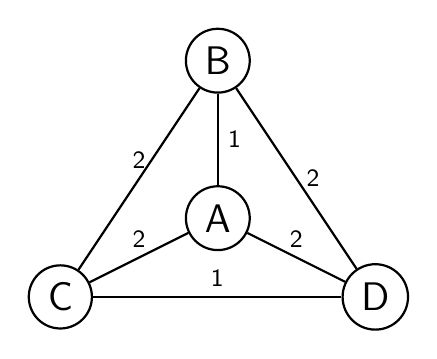
\begin{tikzpicture}[auto,node distance=3cm, every loop/.style={},thick,main node/.style={circle,draw,font=\sffamily\Large}]
			\node[main node] at (0, 0) (a) {A};
			\node[main node] at (0, 2) (b) {B};
			\node[main node] at (-2, -1) (c) {C};
			\node[main node] at (2, -1) (d) {D};

			\path[every node/.style={font=\sffamily\small}]
				(a) edge[] node [right] {1} (b)
				(a) edge node [above] {2} (c)
				(a) edge node [above] {2} (d)
				(b) edge node [right] {2} (d)
				(b) edge node [above] {2} (c)
				(c) edge node [above] {1} (d)
				;
		\end{tikzpicture}
	}
	\caption{Exemplo}
	\label{graph}
\end{wrapfigure}

O nome do problema está relacionado ao problema do planejamento de rotas de carteiros: dada uma cidade com várias ruas de diferentes comprimentos e um posto de carteiros, encontrar a menor rota que um carteiro deve percorrer de modo a passar por todas ruas da cidade entregando cartas e voltar ao posto de carteiros no fim de sua rota.

Entre outras aplicações do problema estão o planejamento de rotas de coletadores de lixo e removedores de neve\footnote{Na cidade de Morris, em Minnesota, Estados Unidos, foi realizado um estudo para otimizar as rotas de removedores de neve baseado no Problema do Carteiro Chinês \cite{snow-removal}}.

Por exemplo, para a figura \ref{graph}, um passeio fechado de custo ótimo seria: 

\[ \{A, B, D, C, A, D, C, B, A\} \] 

Sendo este um caminho fechado de custo 12.
Neste exemplo foi necessário que as arestas $AB$ e $DC$ fossem percorridas duas vezes no passeio, porém nem sempre é necessária esta repetição.

No caso em que o grafo tratado é euleriano, a resposta para o problema do carteiro chinês é justamente o circuito euleriano do grafo.
Nos outros casos, sendo o grafo conexo, o procedimento que seguiremos será a realizar a cópia de algumas arestas do grafo de modo a torná-lo euleriano.

A solução do PCC para um grafo $G$ terá duas partes: Tornar $G$ euleriano com o menor custo possível, criando cópias de arestas existentes e encontrar o ciclo euleriano do grafo $G$ modificado.

Uma generalização do Problema do Carteiro Chinês é o \textbf{problema das T-junções}.
Este problema consiste em, dado um grafo $(V, E)$ e um conjunto de vértices $T \subseteq V$, definir um conjunto de arestas $J$ de custo mínimo tal que todo vértice do conjunto $T$ possui grau ímpar no grafo $(V, J)$ e todo vértice em $V \setminus T$ possui grau par no mesmo grafo.

Se tomamos, por exemplo, $T$ como o conjunto de vértices de grau ímpar em um grafo não direcionado, um T-join $J$ de menor custo representa exatamente o conjunto de arestas que, se adicionadas a um grafo qualquer torna-o euleriano.
Sendo assim, o problema das T-junções resolve a primeira parte do PCC: tornar um grafo euleriano com o menor custo possível. 
Por esse motivo podemos dizer que o problema das T-junções é uma generalização do problema do carteiro chinês.

Discutiremos nas seções a seguir a solução para o problema em questão com base nas especificidades do grafo do problema. 
Desconsideraremos nas análises a seguir grafos que possuam vértices isolados, isto é, vértices que não possuam arestas, já que tais vértices não afetam a solução do problema.

\subsection{Grafos não direcionados}
        \label{sec:pcc}

Analisaremos o caso em que o problema é modelado a partir de um grafo $G(V, E)$ simples, conexo e não direcionado.

Uma solução qualquer $T$ do problema do carteiro chinês deverá percorrer cada aresta de $G$ pelo menos uma vez, sendo assim uma trilha fechada.
Se $G$ é euleriano, então uma solução para o PCC é o próprio circuito euleriano do grafo.
Do contrário, será necessário que $T$ percorra pelo menos uma aresta multiplas vezes.

Seja $1 + x_e$ o número de vezes que uma aresta $e \in E$ é percorrida em $T$.
Definimos $G'$ como o grafo formado por $G$ adicionado de $x_e$ cópias de cada aresta $e \in E$. 
Isto é, cada aresta $e$ de $G$ aparecerá em $G'$ $1 + x_e$ vezes e a trilha fechada $T$ (solução do PCC em $G$) percorre cada uma dessas arestas uma única vez.
Por definição $G'$ será euleriano, e a trilha euleriana de $G'$ corresponderá à $T$, solução do PCC para o grafo $G$.

Sendo assim, podemos separar a solução do PCC em duas partes: Encontrar o valor ótimo de $x_e$ para o problema descrito e, em seguida, encontrar um circuito euleriano no grafo $G'$ construido.

Resolveremos a primeira parte do problema com um algoritmo de emparelhamento.

%Seja $E(v)$ o conjunto de arestas ligadas ao vértice $v \in V$, e seja $c_e$ o custo de se percorrer uma aresta $e \in E$, que deverá ser não-negativo.

%Encontrar uma solução ótima para o PCC é equivalente a encontrar os valores inteiros e não negativos $x_e$ tal que $\sum_{e\in E(u)}(1 + x_e) \equiv 0 \mod 2$ para todo $u \in V$, minimizando o valor de $\sum_e c_ex_e$.

\begin{lemma} 
    \label{lemma-pcc}
    Para todo grafo simples e conexo, existe uma solução ótima do PCC em que cada aresta é copiada no máximo 1 vez, ou seja que $x_e$ vale 0 ou 1. 
\end{lemma}

\begin{proof}
    Seja $T$ uma solução ótima do PCC para um grafo $G$ e $x$ um vetor indicando a quantidade de cópias necessárias de cada aresta de $G$ para a solução $T$. 
    Sabemos que $x$ deverá possuir valores inteiros não negativos, além disso, sabemos que o grafo $G'$, induzido por $x$, deverá ser euleriano e que o valor de $\sum_e c_ex_e$ será mínimo.

    Seja $x^*$ um vetor definido do seguinte modo:

    \[  x^*_e = x_e \bmod 2    \]

    Como o grafo $G'$ induzido por $x$ era euleriano, o grafo $G^*$ induzido por $x^*$ também deverá ser euleriano, pois a paridade dos vértices em ambos grafos é a mesma, e também pois tanto $G'$ quanto $G^*$ possuem $G$, que é conexo, como um subgrafo, e portanto também são conexos.
    
    Pela definição, $G^*$ usa um número menor ou igual de arestas duplicadas que $G'$, fazendo com que o seguinte se mantenha: $\sum_e c_ex^*_e \leq \sum_e c_ex_e$.

    No entanto, como $x$ foi derivado da solução ótima $T$, sabemos que $\sum_e c_ex_e$ deverá ser mínimo, e portanto, $\sum_e c_ex^*_e = \sum_e c_ex_e$. 

    Sendo assim, os valores de $x^*$ serão apenas 0 ou 1, por definição, e $T^*$ consistirá em uma solução ótima, assim como $T$, provando o lema.

\end{proof}

\begin{lemma}
    Para todo grafo $G$ simples e conexo, existe uma solução ótima do PCC cujo conjunto de arestas duplicadas consiste na união de caminhos aresta-disjuntos entre vértices de grau ímpar.
\end{lemma}

\begin{proof}

    Inicialmente trataremos o caso em que $G$ não possui nenhum vértice de grau ímpar:
    Se todos vértices de $G$ tem grau par, então o mesmo deve possuir um circuito euleriano. 
    Por isso, o vetor $x' = \{0, 0, \dots, 0\}$ induz uma solução válida para o PCC, e possui custo zero, sendo assim esta uma solução ótima.
    Como o conjunto de arestas duplicadas nesta solução é vazio, vale o lema para este grafo.

    Provado este caso, seguiremos a demonstração assumindo que $G$ possui ao menos um vértice de grau ímpar.

    Seja $T$ uma solução ótima do PCC para um grafo $G(V, E)$  em que cada aresta é copiada no máximo 1 vez, ou seja que $x_e$ valerá 0 ou 1. 
    A existência de tal solução é garantida pelo lema \ref{lemma-pcc}.
    Realizaremos uma prova por indução no número de arestas duplicadas de $G$, ou seja, em $\sum_e x_e$, para toda aresta $e \in E$. 

    O caso base dessa indução é quando $\sum_e x_e = 0$. 
    Neste caso, o conjunto de arestas duplicadas será vazio, valendo então a propriedade do lema.

    A hipótese de indução será que a propriedade do lema vale para uma soma $\sum_e x_e < k$, com $k > 0$.

    Analisaremos agora a situação em que $\sum_e x_e = k$, com $k > 0$.

    Seja $v$ um vértice de $G$ de grau ímpar,  $C$ um caminho de tamanho maximal que começa no vértice $v$ e percorre apenas arestas duplicadas e seja $G'$ o grafo, possivelmente desconexo, $G$ decrescido das arestas pertencentes a $C$.


    Todos os vértices em $G$ e $G'$ terão a mesma paridade de grau, exceto pelos vértices extremos de $C$. 
    Como estes eram vértices de grau ímpar em $G$ e apenas uma aresta foi retirada dos mesmos, ambos terão grau par em $G'$.

    Sendo assim, podemos definir um vetor $x'$ que induz uma solução ótima para $G'$ do seguinte modo:

    \[ 
        x'_e = 
        \begin{cases} 
            0 & e \in C \\
            x_e & e \notin C 
        \end{cases}
    \]


    Vale também o seguinte:

    \begin{align*}
        \sum_e x'_e &= \sum_e x_e - |\mathcal{C}| \\ 
        \sum_e x'_e &< \sum_e x_e \\
        \sum_e x'_e &< k
    \end{align*}

    Sendo assim, vale a hipótese de indução para o grafo $G'$, ou seja, existe um conjunto $\mathcal{C}$ de caminhos aresta-disjuntos entre vértices de grau ímpar composto por arestas duplicadas (ou seja, para as quais $x'_e = 1$).

    Como o grafo $G'$ não possui as arestas do caminho $C$, temos que todo caminho de $\mathcal{C}$ deverá ser aresta-disjunto com $C$.
    Deste modo, o conjunto de caminhos aresta-disjuntos entre vértices de grau ímpar $\mathcal{C} \cup C$, que induz o grafo $T$, consistirá de uma solução ótima para o PCC em $G$.
    Provando assim o passo da indução.

    Finalizando então a prova por indução do lema.

    \begin{figure}
        \centering
        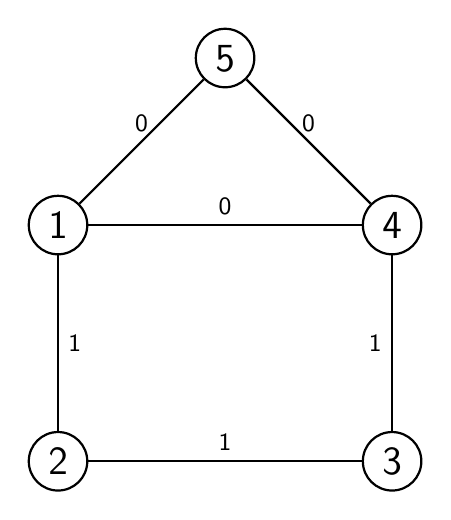
\begin{tikzpicture}[auto,node distance=3cm, every loop/.style={},thick,main node/.style={circle,draw,font=\sffamily\Large}]
            \node[main node] (5) {5};
            \node[main node] (1) [below left of=5]{1};
            \node[main node] (2) [below of=1] {2};
            \node[main node] (4) [below right of=5] {4};
            \node[main node] (3) [below of=4] {3};

          \path[every node/.style={font=\sffamily\small}]
            (5) edge node [above] {0} (1)
            (5) edge node [above] {0} (4)
            (1) edge node [above] {0} (4)
            (2) edge node [right] {1} (1)
            (3) edge node [above] {1} (2)
            (4) edge node [left] {1} (3)
            ;
        \end{tikzpicture}
        \caption{Possível estrutura em grafo com vértices de grau ímpar}
        \label{pcc-case1}
    \end{figure}
    \begin{figure}
        \centering
        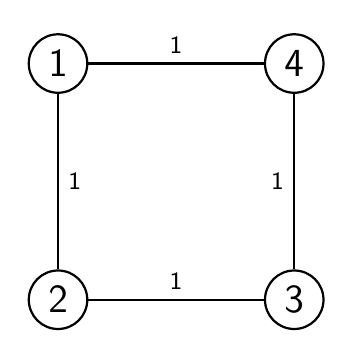
\begin{tikzpicture}[auto,node distance=3cm, every loop/.style={},thick,main node/.style={circle,draw,font=\sffamily\Large}]
            \node[main node] (1) {1};
            \node[main node] (2) [below of=1] {2};
            \node[main node] (4) [right of=1] {4};
            \node[main node] (3) [below of=4] {3};

          \path[every node/.style={font=\sffamily\small}]
            (1) edge node [above] {1} (4)
            (2) edge node [right] {1} (1)
            (3) edge node [above] {1} (2)
            (4) edge node [left] {1} (3)
            ;
        \end{tikzpicture}
        \caption{Caso em que o grafo tratado não possui vértices de grau ímpar}
        \label{pcc-case2}
    \end{figure}

\end{proof}

\begin{lemma}
    \label{lema-final}
    Para todo grafo $G$ simples e conexo, existe uma solução ótima do PCC cujo conjunto de arestas duplicadas é a união de caminhos de custo mínimo entre vértices de grau ímpar.
\end{lemma}

\begin{proof}
    Seja $S$ o conjunto de arestas duplicadas em uma solução ótima do PCC para o grafo $G$, que consiste de uma união de caminhos aresta-disjuntos entre vértices de grau ímpar.

    Imagine que um caminho $C$ pertencente a $S$, que liga os vértices quaisquer $u$ e $v$, não é o caminho mínimo entre os vértices que liga. 
    Isto é, existe um caminho $C'$ de custo menor que $C$ que liga $u$ e $v$.

    Neste caso, poderiamos retirar de $S$ as arestas do caminho $C$ e adicionar ao conjunto as arestas de $C'$. Deste modo, o conjunto $S$ possuiria um custo menor que o original, nos permitindo derivar de $S$ uma solução para o PCC de custo menor que a solução original.

    Porém, fazia parte da hipótese que a solução original era ótima, nos levando assim a uma contradição.

    Provamos assim o lema, garantindo a existência de uma solução para o PCC que consiste de uma união de caminhos mínimos entre vértices de grau ímpar.

\end{proof}

Um algoritmo que soluciona o problema se baseia em criar um novo grafo completo $G'(V', E')$. 
$V'$ é definido como o subconjunto de vértices de $V$ que possuem um grau ímpar em $G$. 
O custo de uma aresta de $E'$ entre dois vértices $u$ e $v$ quaisquer será o custo de um caminho mínimo entre $u$ e $v$ no grafo original $G$.


Pelo lema \ref{lema-final}, uma solução ótima do PCC em $G$ possui um conjunto de arestas duplicadas que pode ser representado como a união de caminhos de custo mínimo entre vértices de grau ímpar. 
Como $V'$ é o conjunto dos vértices de grau ímpar em $G$ e cada aresta de $E'$ representa um caminho de custo mínimo entre dois vértices de $V'$, podemos reduzir o problema original a um problema de emparelhamento perfeito de custo mínimo no grafo $G'$.

Dado um emparelhamento perfeito $M$ em $G'$ de custo mínimo, é possível derivar uma solução ótima do PCC. Esta solução será dada por um circuito euleriano no grafo $G^*$ que construímos abaixo:

Considere $G^* = (V, E)$. Agora, para cada aresta $e = uv \in M$ (emparelhamento de $G'$), tome $C$ um caminho de custo mínimo de $u$ a $v$ em $G$ e faça $G^* \leftarrow G^* \cup C$, ou seja, duplique as arestas de $C$ em $G^*$.

A duplicação das arestas de um caminho modifica apenas a paridade de grau dos vértices extremos.
Como, no procedimento acima, estamos duplicando as arestas de todos caminhos derivados do emparelhamento perfeito $M$, isso implica que modificamos as paridades dos graus de todos os vértices de $G^*$, ou seja, modificamos apenas as paridades dos graus dos vértices de grau ímpar de $G$.

Sendo assim, o grafo $G^*$ resultante é euleriano, e a solução para o PCC do grafo $G$ é o circuito euleriano de $G^*$.


Segue no algoritmo \ref{pcc-pseudocode} uma versão em pseudo-código do algoritmo descrito.



    % TODO: Expandir nesses assuntos:
        % Complexidade de um algoritmo
		%\item Essa solução não se aproveita do grafo ser esparso, há outra formulação do Edmonds e Johnson que leva isso em consideração.
		%\item Um problema similar é o de cobrir todas arestas com ciclos simples, de modo que o comprimento total dos ciclos é minimizado. Para grafos planares esses problemas são equivalentes.


    \begin{algorithm}
    \floatname{algorithm}{Algoritmo}%
    \caption{Solução do PCC em grafos não direcionados}
    \label{pcc-pseudocode}
    \begin{algorithmic}[1]
    \Function{pcc}{G}
    \State $(V, E, dist) \gets G$
    \State $V' \gets \{v \in V : \delta[v] $ é impar$\}$
    \State $dist' \gets $ FLOYD\_WARSHALL$(V, E, dist)$
    \State $E' \gets V' \times V'$
    \State $G' \gets (V', E', dist')$
    \State $M \gets $ EMPARELHAMENTO\_PERFEITO\_MINIMO$(G')$
    \State $E^* \gets E$
    \For{$uv \in M$}
        \State $C \gets$ EXPANDE$(uv, E, dist, dist')$
        \State $E^* \gets E^* \cup C$
    \EndFor
    \State $G^* \gets (V, E^*)$
    \State \Return CIRCUITO\_EULERIANO$(G^*)$
    \EndFunction 

    \Function{expande}{uv, E, dist, dist'}
    \If{$u = v$}
    \Return $\emptyset$
    \EndIf
    \For{$w : uw \in E$}
        \If{dist'[u][v] = dist[u][w] + dist'[w][v]} 
        \State \Return $\{uw\}$  $\cup$ EXPANDE$(wv, E, dist, dist')$
        \EndIf
    \EndFor
    \EndFunction

    \end{algorithmic}
    \end{algorithm}

Escolheu-se o algoritmo de Floyd-Warshall para encontrar as distâncias mínimas entre todo par de vértices de $G$.
Apesar de tal algoritmo possuir complexidade $\mathcal{O}(|V|^3)$, ele possui uma simples implementação.

Se $G$ não possuir arestas de custo negativo, uma alternativa ao algoritmo de Floyd-Warshall é utilizar o algoritmo de Dijkstra $|V'|$ vezes, calculando a distância mínima de cada vértice de grau ímpar a todos outros vértices do grafo, possuindo assim uma complexidade $\mathcal{O}(|V'||E|\log|V|)$. 

Uma solução para se encontrar o emparelhamento perfeito mínimo de um grafo não direcionado com custos é usar o algoritmo Blossom de Edmonds\cite{blossom}. 
Encontra-se nas referências deste trabalho uma implementação do algoritmo de Edmonds intitulada ``Blossom V'' e publicada por Vladimir Kolmogorov em 2009\cite{kolmogorov}.

    \subsection{Grafos direcionados}

    Analisaremos agora o problema do carteiro chinês aplicado a digrafos.

    \begin{lemma}
        Um digrafo $G$ possui solução para o problema do carteiro chinês se, e somente se, é fortemente conexo.
    \end{lemma}

    \begin{proof}


        ($\Rightarrow$) Começamos provando que para que um digrafo $G$ possua solução para o problema do carteiro chinês é necessário que o mesmo seja fortemente conexo.

        Vamos assumir, por absurdo, que $G$ possui uma solução para o PCC mas não é fortemente conexo.

        Como $G$ possui uma solução para o PCC, então existe um passeio fechado $T$ que passa por todos arcos de $G$.

         Além disso, como $T$ é um passeio fechado, para cada par de vértices $u, v$ de $G$, sabemos que $T$ passa por $u$ e $v$.
         Assim, $T = \{ v_0, v_1, \dots, v_i = u, \dots, v_j = v, \dots \}$.

        A partir de um passeio entre dois vértices sempre é possível derivar um caminho entre os mesmos seguindo o seguinte método:

        \begin{tcolorbox}
            \textbf{Método para derivar um caminho de um passeio qualquer}
            
            Seja $P$ um passeio que liga dois vértices quaisquer, mostraremos como construir um caminho ligando esses mesmos vértices a partir de $P$.

            Como $P$ é um passeio, possivelmente ele percorre um mesmo vértice mais que uma vez. Do contrário, já podemos considerar $P$ um caminho, finalizando o método. 

            Enquanto houver um vértice $v$ percorrido mais que uma vez por $P$ executa-se o seguinte passo:
    

            Retiramos de $P$ todos os vértices entre a primeira e a última aparição do vértice $v$, mantendo apenas tal vértice: 


            Portanto um passeio $P$ qualquer com repetição do vértice $v$, como o seguinte:
            \[
                P = \{ u_1, \dots u_i, v, \dots, v, u_j, \dots u_n\}
            \]

            Passa a ser:


            \[
                P = \{ u_1, \dots u_i, v, u_j, \dots u_n\}
            \]

            Repete-se tal passo até que $P$ não percorra um mesmo vértice duas vezes, se tornando assim, por definição, um caminho.

        \end{tcolorbox}
         
        Sendo assim, afirmamos que todo par de vértices presentes em $T$ possui um caminho entre si.

        Já que não estamos considerando neste trabalho digrafos que possuem vértices isolados, cada vértice de $G$ deve ser incidente ao menos a um arco. Além disso, como todos arcos são percorridos em $T$, já que ele é uma solução do PCC, todos os vértices deverão estar presentes no passeio fechado $T$.
        Por consequência para todo par de vértices de $G$ existe um caminho entre eles o que define $G$ como um grafo fortemente conexo, contradizendo a hipótese inicial.

        Provando assim que um digrafo que possua solução para o PCC é necessariamente fortemente conexo. 

        ($\Leftarrow$)  Provaremos agora que todo grafo fortemente conexo $G$ possui uma solução para o PCC.

        Seja $v$ um vértice qualquer de $G$. Podemos construir uma solução $P$ para o problema do carteiro chinês do seguinte modo:


        Para qualquer arco $uw$ de $G$ definimos um circuito $C_{uw}$ que passa por $uw$ e pelo vértice $v$ como a concatenação do caminho de $v$ a $u$, do arco $uw$ e do caminho de $w$ a $v$.
        
        A existência de um caminho entre quaisquer dois vértices é garantida, já que $G$ é fortemente conexo, garantindo assim a existência de $C_{uw}$.
        
        Para construir a solução $P$, finalmente, basta realizar a concatenação dos circuitos $C_{e}$ para todo arco $e$ presente em $G$.

        Deste modo garantimos que toda aresta de $G$ é percorrida, provando assim a volta do lema: todo digrafo fortemente conexo possui uma solução para o problema do carteiro chinês.

    \end{proof}

    Em linhas gerais, o algoritmo que soluciona o problema do carteiro chinês para digrafos envolve multiplicar arestas do grafo original até que o mesmo se torne euleriano. O circuito euleriano desse digrafo modificado será a solução do problema do carteiro chinês para o digrafo original, do modo similar à solução para o PCC em grafos não direcionados.
    
    Uma grande diferença na solução do problema do carteiro chinês é que, para digrafos, não vale o lema \ref{lemma-pcc}, que garante a existência de uma solução para todo PCC em que cada aresta do grafo é percorrida no máximo duas vezes.
    Um contra-exemplo disso é o caso ilustrado na figura \ref{counter-lemma}. 

    \begin{figure}[h]
        \centering
        \begin{tikzpicture}[node distance=3cm, every loop/.style={},thick,main node/.style={circle,draw,font=\sffamily\Large}]
            \node[main node] (1) {1};
            \node[main node] (2) [right of=1] {2};
            \draw[edge] (1) to[bend left=50] (2);
            \draw[edge] (1) to[bend right=50] (2);
            \draw[edge] (1) to[] (2);
            \draw[edge] (2) to[bend left=100] (1);
        \end{tikzpicture}
        \caption{Contra exemplo do lema \ref{lemma-pcc} para os digrafos}
        \label{counter-lemma}
    \end{figure}

    Para que um passeio fechado percorra os três arcos de $1$ a $2$ da figura \ref{counter-lemma}, é necessário que esse mesmo passeio percorra três vezes o arco de $2$ a $1$.

    O lema \ref{lemma-pcc} é utilizado para justificar a utilização de um algoritmo de emparelhamento perfeito para definir quais arestas duplicar na solução do PCC.
    Como tal lema não vale para digrafos, a escolha dessas arestas deverá ser feita de um modo diferente, utilizando um algoritmo de fluxo máximo de custo mínimo, como veremos a seguir, no detalhamento do algoritmo que soluciona o PCC.

    A solução do PCC para um digrafo $G$ fortemente conexo pode ser dividida em 4 passos:

    \begin{enumerate}
        \item[\textbf{1º}] Define-se $F$ como o conjunto dos vértices que possuam grau de entrada ($\delta^+$) maior que o grau de saída ($\delta^-$) e $S$ como o conjunto dos vértices que possuam grau de saída maior que o grau de entrada.

        Calcula-se o custo do menor caminho entre todos os pares de vértices $u, v$ onde $u \in F$ e $v \in S$.

        \item[\textbf{2º}] Modela-se um problema de transporte: 
        Seja $b$ uma função demanda definida para todo vértice como $b(v) = \delta^-(v) - \delta^+(v)$.
        Os vértices de $F$ serão vértices de oferta (com função demanda $b$ negativa), cada vértice $u \in F$ terá que escoar $-b(u)$ unidades de fluxo. 
        Já os vértices de $S$ serão vértices de demanda, cada vértice $v \in S$ terá que receber $b(v)$ unidades de fluxo.

        Todo par de vértices $u, v$ com $u \in F$ e $v \in S$ será ligado por um arco que pode transportar qualquer quantidade de fluxo, mas que tem custo igual ao custo de um menor caminho de $u$ a $v$ por unidade de fluxo transportada, calculado no primeiro passo.

        Deve-se resolver tal problema de transporte no grafo $F,S$-bipartido minimizando o custo total e respeitando a função demanda definida.

        \item[\textbf{3º}] Usa-se a solução do problema de transporte para criar um digrafo euleriano $G^*$ a partir de $G$.
            Inicialmente $G^* = G$.

            Uma solução do problema de transporte descrito será uma função $f: F\times S \rightarrow \mathbb{N}$ que determina a quantidade de fluxo transportada entre cada par de vértices de $F$ e $S$.

            Se um arco $uv$ é escolhido para transportar uma quantidade $f(uv)$ positiva de fluxo, deve-se criar $f(uv)$ cópias de todos arcos do menor caminho de $u$ a $v$ em $G^*$, chamaremos esse processo de expansão de $uv$.

            Após a duplicação dos arcos de um caminho entre dois vértices $u$ e $v$ a diferença absoluta dos graus de entrada e saída de $u$ e $v$ diminuirão em uma unidade, essa mesma diferença de graus se manterá constante para vértices internos ao caminho. 

            Ao final da expansão de todos arcos que possuem $f$ positivo, todos vértices de $G^*$ possuirão um mesmo valor de grau de entrada e saída, tornando $G^*$ euleriano pelo teorema \ref{euler-digraph}.

        \item[\textbf{4º}] Encontrar o circuito euleriano de $G^*$, que será também a solução do problema do carteiro chinês para o grafo original $G$.

    \end{enumerate}


    O algoritmo \ref{di-pcc-pseudocode} é a implementação em pseudo-código da solução descrita acima.

    Na função $PROBLEMA\_DE\_TRANSPORTE$ define-se uma redução do problema para o problema do fluxo máximo de custo mínimo. 
    Para se resolver esta redução, pode-se utilizar um algoritmo de Simplex para Redes como discutido por Orlin \cite{network-simplex}, de complexidade $\mathcal{O}(VE\log V\log(VC))$, sendo $C$ a capacidade máxima dos arcos da rede. 
    Outra solução para a redução é usar uma variação do algoritmo de Edmonds-Karp \cite{edmonds-karp} para fluxo de custo mínimo de complexidade $\mathcal{O}(V^2E^2)$. 
    A explicação e implementação dessa variação estão disponíveis online, no site E-maxx \cite{min-cost}. 

    \begin{algorithm}
    \floatname{algorithm}{Algoritmo}%
    \caption{Solução do PCC em digrafos}
    \label{di-pcc-pseudocode}
    \begin{algorithmic}[1]
    \Function{pcc}{G}
    \State $(V, E, dist) \gets G$
    \State $dist' \gets $ FLOYD\_WARSHALL$(V, E, dist)$
    \For{$v \in V$}
        \State $b(v) \gets \delta^-(v) - \delta^+(v)$ \Comment Calcula a função demanda
    \EndFor
    \State $F \gets \{v \in V : b(v) < 0\}$
    \State $S \gets \{v \in V : b(v) > 0\}$
    \State $f \gets $ PROBLEMA\_DE\_TRANSPORTE$(F, S, dist, b)$
    \State $E^* \gets E$ \Comment{Cria uma cópia de $E$}
    \For{$uv \in E$}
        \State $C \gets$ EXPANDE$(uv, E, dist, dist')$
        \For{$i$ de $1$ a $f(uv)$} 
            \State $E^* \gets E^* \cup C$ \Comment Duplica $f(uv)$ vezes os arcos de $C$ 
        \EndFor
    \EndFor
    \State $G^* \gets (V, E^*)$
    \State \Return CIRCUITO\_EULERIANO$(G^*)$
    \EndFunction 

    \Function{expande}{uv, E, dist, dist'}
    \If{$u = v$}
    \Return $\emptyset$
    \EndIf
    \For{$w : uw \in E$}
        \If{dist'[u][v] = dist[u][w] + dist'[w][v]} 
        \State \Return $\{uw\}$  $\cup$ EXPANDE$(wv, E, dist, dist')$
        \EndIf
    \EndFor
    \EndFunction

    \Function{problema\_de\_transporte}{F, S, custo, b}
        \State Define dois vértices artificiais, uma fonte $s$ e um sorvedouro $t$
        \State $E \gets F\times S$
        \For{$uv \in E$}
            \State $cap(uv) = \infty$
        \EndFor
        \For{$u \in F$}
            \State $cap(su) = -b(u)$
            \State $custo(su) = 0$
            \State $E = E \cup \{su\}$
        \EndFor
        \For{$v \in S$}
            \State $cap(vt) = b(v)$
            \State $custo(vt) = 0$
            \State $E = E \cup \{vt\}$
        \EndFor
        \State \Return FLUXO\_CUSTO\_MINIMO$(s, t, E, custo, cap)$
    \EndFunction
    \end{algorithmic}
    \end{algorithm}

    Aplicaremos agora o passo a passo apresentado acima em um exemplo. 

    \begin{figure}[H]
        \centering
        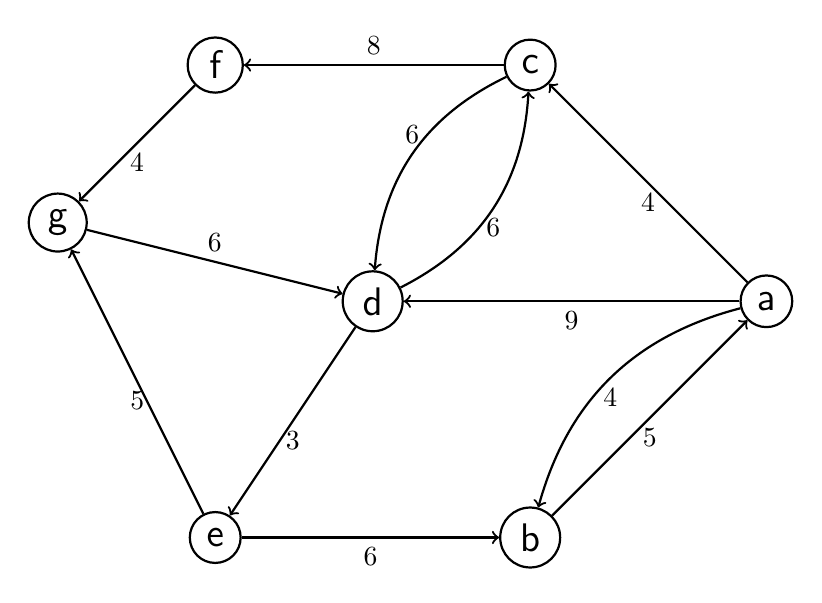
\begin{tikzpicture}[node distance=3cm, every loop/.style={},thick,main node/.style={circle,draw,font=\sffamily\Large}]

            \node[main node] (d) {d};
            \node[main node] at (-4, 1) (g) {g};
            \node[main node] at (-2, 3) (f) {f};
            \node[main node] at (2, 3) (c) {c};
            \node[main node] at (5, 0) (a) {a};
            \node[main node] at (-2, -3) (e) {e};
            \node[main node] at (2, -3) (b) {b};

            \path[->] (a) edge[bend right, below] node {4} (b);
            \path[->] (a) edge[below] node {9} (d);
            \path[->] (a) edge[below] node {4} (c);
            \path[->] (b) edge[below] node {5} (a);
            \path[->] (c) edge[bend right, above] node {6} (d);
            \path[->] (c) edge[above] node {8} (f);
            \path[->] (d) edge[below] node {3} (e);
            \path[->] (d) edge[bend right, below] node {6} (c);
            \path[->] (e) edge[below] node {6} (b);
            \path[->] (e) edge[below] node {5} (g);
            \path[->] (f) edge[below] node {4} (g);
            \path[->] (g) edge[above] node {6} (d);
        \end{tikzpicture}
        \caption{Digrafo retirado de exercício do site do MIT\cite{mit}}
        \label{mit-ex}
    \end{figure}


    \begin{itemize}
        \item[\textbf{1º}] 
            Definimos então os conjuntos $F$ e $S$:

            \[
                F  = \{b, d, g\}
            \]
            \[
                S =  \{a, e\}
            \]

            Computamos também a distância mínima entre os pares de vértices dos dois conjuntos:

            \begin{center}
                \begin{tabular}{ |p{1cm}||p{1cm}|p{1cm}|  }
                    \hline
                     & a & e \\
                    \hline
					\hline
                    b & 4 & 17 \\
                    \hline
                    d & 14 & 3 \\
                    \hline
                    g & 20 & 9\\
                    \hline
                \end{tabular}
            \end{center}

        \item[\textbf{2º}]

            Modelamos então o problema de transporte, os vértices $b, d, g$ escoando uma unidade de fluxo cada e os vértices $a, b$ com demandas 2 e 1, respectivamente.

            \begin{figure}[H]
                \centering
                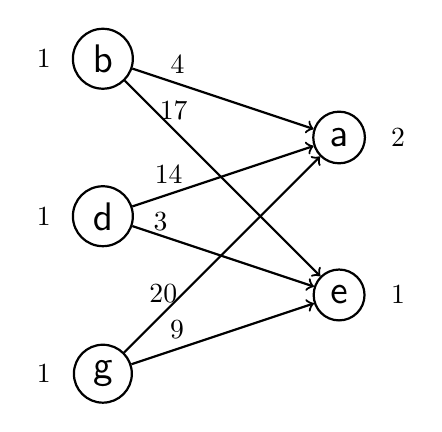
\begin{tikzpicture}[node distance=3cm, every loop/.style={},thick,main node/.style={circle,draw,font=\sffamily\Large}]

					\node[main node] (1) {b};
					\node (v1) at(-0.75, 0) {1};
					\node[main node] at (0, -2) (2) {d};
					\node (v2) at(-0.75, -2) {1};
					\node[main node] at (0, -4) (3) {g};
					\node (v3) at(-0.75, -4) {1};

					\node[main node] at(3, -1) (4) {a};
					\node (v4) at(3.75, -1) {2};
					\node[main node] at(3, -3) (5) {e};
					\node (v5) at(3.75, -3) {1};

                    \path[->] (1) edge node[pos=0.25,above] {4} (4);
                    \path[->] (1) edge node[pos=0.25,above] {17} (5);
                    \path[->] (2) edge node[pos=0.20,above] {14} (4);
                    \path[->] (2) edge node[pos=0.25,above left] {3} (5);
                    \path[->] (3) edge node[pos=0.20,above] {20} (4);
                    \path[->] (3) edge node[pos=0.25,above] {9} (5);
                \end{tikzpicture}
            \end{figure}

            Os arcos definidos entre os vértices de $F$ e $S$ possuem capacidade infinita e custo igual à distância mínima dos mesmos vértices em $G$, como já calculado no primeiro passo.

            Uma solução ótima para o problema apresentado consiste em transportar uma unidade de fluxo pelos arcos de custo $4, 14$ e $9$, escoando os vértices $b, d$ e $g$ e suprindo a demanda dos vértices $a$ e $e$.

            \begin{figure}[H]
                \centering
                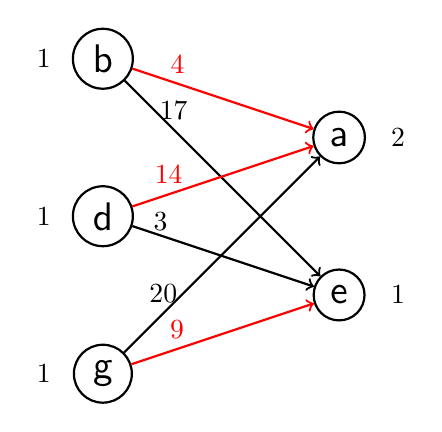
\begin{tikzpicture}[node distance=3cm, every loop/.style={},thick,main node/.style={circle,draw,font=\sffamily\Large}]

					\node[main node] (1) {b};
					\node (v1) at(-0.75, 0) {1};
					\node[main node] at (0, -2) (2) {d};
					\node (v2) at(-0.75, -2) {1};
					\node[main node] at (0, -4) (3) {g};
					\node (v3) at(-0.75, -4) {1};

					\node[main node] at(3, -1) (4) {a};
					\node (v4) at(3.75, -1) {2};
					\node[main node] at(3, -3) (5) {e};
					\node (v5) at(3.75, -3) {1};

                    \path[->] (1) edge[red] node[pos=0.25,above] {4} (4);
                    \path[->] (1) edge node[pos=0.25,above] {17} (5);
                    \path[->] (2) edge[red] node[pos=0.20,above] {14} (4);
                    \path[->] (2) edge node[pos=0.25,above left] {3} (5);
                    \path[->] (3) edge node[pos=0.20,above] {20} (4);
                    \path[->] (3) edge[red] node[pos=0.25,above] {9} (5);
                \end{tikzpicture}
            \end{figure}

        \item[\textbf{3º}] Agora devemos realizar a duplicação dos caminhos representados pelos arcos $ba, da$ e $ge$.

            Representamos o estado inicial do digrafo $G$, sem os pesos nos arcos:

            \begin{figure}[H]
                \centering
                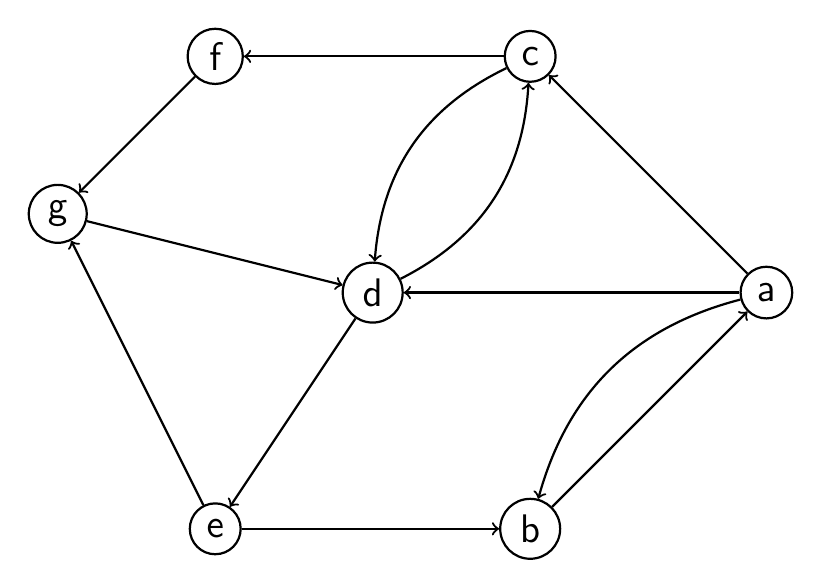
\begin{tikzpicture}[node distance=3cm, every loop/.style={},thick,main node/.style={circle,draw,font=\sffamily\Large}]

					\node[main node] (d) {d};
					\node[main node] at (-4, 1) (g) {g};
					\node[main node] at (-2, 3) (f) {f};
					\node[main node] at (2, 3) (c) {c};
					\node[main node] at (5, 0) (a) {a};
					\node[main node] at (-2, -3) (e) {e};
					\node[main node] at (2, -3) (b) {b};

					\path[->] (a) edge[bend right, below] node {} (b);
					\path[->] (a) edge[below] node {} (d);
					\path[->] (a) edge[below] node {} (c);
					\path[->] (b) edge[below] node {} (a);
					\path[->] (c) edge[bend right, above] node {} (d);
					\path[->] (c) edge[above] node {} (f);
					\path[->] (d) edge[below] node {} (e);
					\path[->] (d) edge[bend right, below] node {} (c);
					\path[->] (e) edge[below] node {} (b);
					\path[->] (e) edge[below] node {} (g);
					\path[->] (f) edge[below] node {} (g);
                    \path[->] (g) edge[above] node {} (d);
                \end{tikzpicture}
            \end{figure}

            Faremos tal duplicação passo a passo, começando a duplicar os arcos do caminho mínimo de $b$ a $a$. Representamos os arcos adicionados em vermelho.


            \begin{figure}[H]
                \centering
                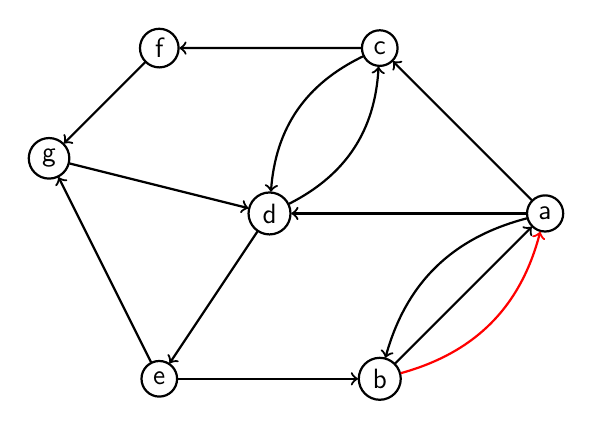
\begin{tikzpicture}[scale=0.7, every node/.style={scale=0.7},node distance=3cm, every loop/.style={},thick,main node/.style={circle,draw,font=\sffamily\Large}]

					\node[main node] (d) {d};
					\node[main node] at (-4, 1) (g) {g};
					\node[main node] at (-2, 3) (f) {f};
					\node[main node] at (2, 3) (c) {c};
					\node[main node] at (5, 0) (a) {a};
					\node[main node] at (-2, -3) (e) {e};
					\node[main node] at (2, -3) (b) {b};

					\path[->] (a) edge[bend right, below] node {} (b);
					\path[->] (a) edge[below] node {} (d);
					\path[->] (a) edge[below] node {} (c);
					\path[->] (b) edge[below] node {} (a);
					\path[->] (b) edge[red, bend right, below] node {} (a);
					\path[->] (c) edge[bend right, above] node {} (d);
					\path[->] (c) edge[above] node {} (f);
					\path[->] (d) edge[below] node {} (e);
					\path[->] (d) edge[bend right, below] node {} (c);
					\path[->] (e) edge[below] node {} (b);
					\path[->] (e) edge[below] node {} (g);
					\path[->] (f) edge[below] node {} (g);
                    \path[->] (g) edge[above] node {} (d);
                \end{tikzpicture}
            \end{figure}

    Agora duplicaremos os arcos do caminho mínimo de $d$ a $a$:

    \begin{figure}[H]
        \centering
        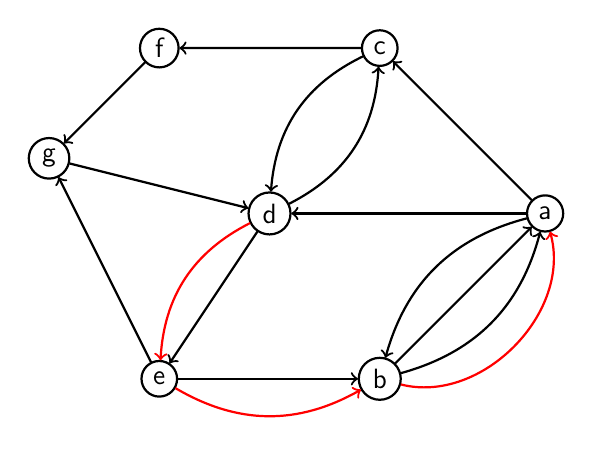
\begin{tikzpicture}[scale=0.7, every node/.style={scale=0.7},node distance=3cm, every loop/.style={},thick,main node/.style={circle,draw,font=\sffamily\Large}]

            \node[main node] (d) {d};
            \node[main node] at (-4, 1) (g) {g};
            \node[main node] at (-2, 3) (f) {f};
            \node[main node] at (2, 3) (c) {c};
            \node[main node] at (5, 0) (a) {a};
            \node[main node] at (-2, -3) (e) {e};
            \node[main node] at (2, -3) (b) {b};

            \path[->] (a) edge[bend right, below] node {} (b);
            \path[->] (a) edge[below] node {} (d);
            \path[->] (a) edge[below] node {} (c);
            \path[->] (b) edge[below] node {} (a);
            \path[->] (b) edge[bend right, below] node {} (a);
            \path[->] (b) edge[red, bend right=60, below] node {} (a);
            \path[->] (c) edge[bend right, above] node {} (d);
            \path[->] (c) edge[above] node {} (f);
            \path[->] (d) edge[below] node {} (e);
            \path[->] (d) edge[red, bend right, below] node {} (e);
            \path[->] (d) edge[bend right, below] node {} (c);
            \path[->] (e) edge[below] node {} (b);
            \path[->] (e) edge[red, bend right, below] node {} (b);
            \path[->] (e) edge[below] node {} (g);
            \path[->] (f) edge[below] node {} (g);
            \path[->] (g) edge[above] node {} (d);
        \end{tikzpicture}
    \end{figure}

    Finalmente, duplicamos os arcos do caminho mínimo de $g$ a $e$:


    \begin{figure}[H]
        \centering
        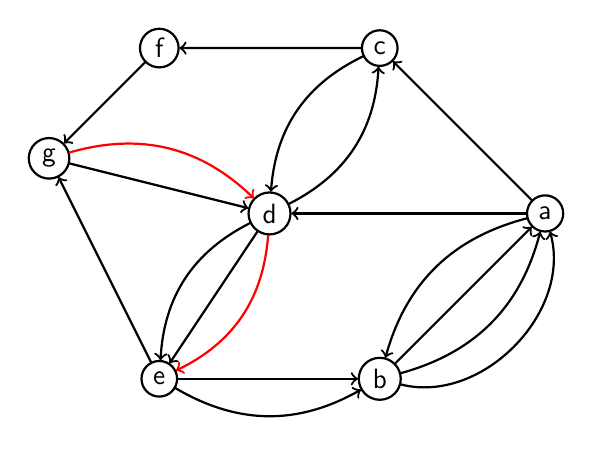
\begin{tikzpicture}[scale=0.7, every node/.style={scale=0.7},node distance=3cm, every loop/.style={},thick,main node/.style={circle,draw,font=\sffamily\Large}]

            \node[main node] (d) {d};
            \node[main node] at (-4, 1) (g) {g};
            \node[main node] at (-2, 3) (f) {f};
            \node[main node] at (2, 3) (c) {c};
            \node[main node] at (5, 0) (a) {a};
            \node[main node] at (-2, -3) (e) {e};
            \node[main node] at (2, -3) (b) {b};

            \path[->] (a) edge[bend right, below] node {} (b);
            \path[->] (a) edge[below] node {} (d);
            \path[->] (a) edge[below] node {} (c);
            \path[->] (b) edge[below] node {} (a);
            \path[->] (b) edge[bend right, below] node {} (a);
            \path[->] (b) edge[bend right=60, below] node {} (a);
            \path[->] (c) edge[bend right, above] node {} (d);
            \path[->] (c) edge[above] node {} (f);
            \path[->] (d) edge[below] node {} (e);
            \path[->] (d) edge[bend right, below] node {} (e);
            \path[->] (d) edge[red, bend left, below] node {} (e);
            \path[->] (d) edge[bend right, below] node {} (c);
            \path[->] (e) edge[below] node {} (b);
            \path[->] (e) edge[bend right, below] node {} (b);
            \path[->] (e) edge[below] node {} (g);
            \path[->] (f) edge[below] node {} (g);
            \path[->] (g) edge[above] node {} (d);
            \path[->] (g) edge[red, bend left, above] node {} (d);
        \end{tikzpicture}
    \end{figure}

    As sucessivas duplicações de caminho realizadas em $G$ fazem com que todos os vértices possuam grau de saída e entrada iguais. Pelo teorema \ref{euler-digraph} temos que o novo grafo é euleriano. No quarto passo derivaremos um circuito euleriano para o digrafo construído.


\item[\textbf{4º}]  Um possível circuito eulerian $\mathcal{C}$ que se inicia no vértice $a$ é o seguinte:

    \[ 
        \mathcal{C} = \{ a, c, f, g, d, c, d, e, g, d, e, b, a, d, e, b, a, b, a \}
    \]

    Representamos tal circuito no grafo abaixo, indicando em cada arco a ordem em que o mesmo é percorrido:

    \begin{figure}[H]
        \centering
        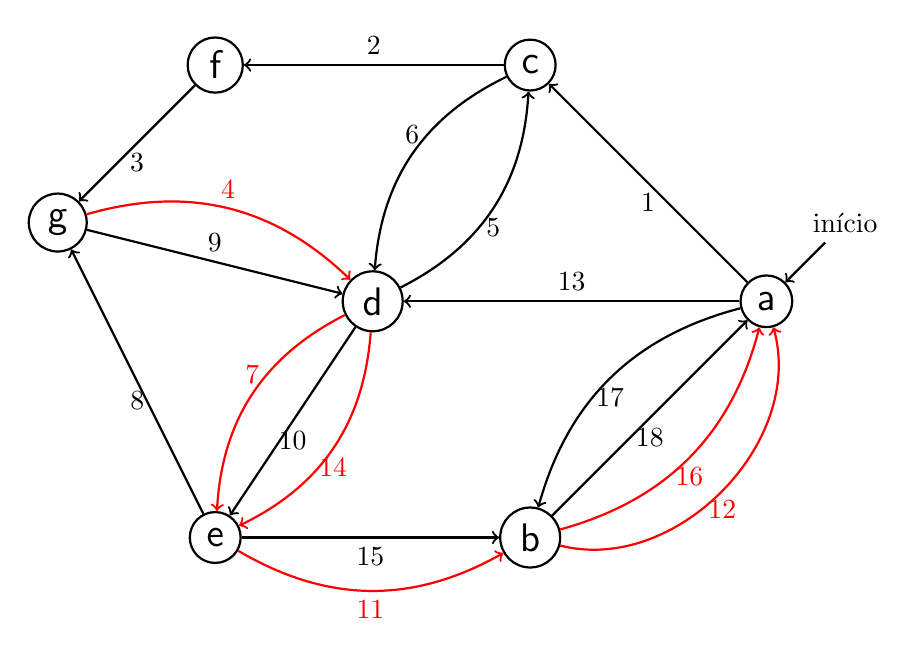
\begin{tikzpicture}[node distance=3cm, every loop/.style={},thick,main node/.style={circle,draw,font=\sffamily\Large}]

            \node[main node] (d) {d};
            \node[main node] at (-4, 1) (g) {g};
            \node[main node] at (-2, 3) (f) {f};
            \node[main node] at (2, 3) (c) {c};
            \node[main node] at (5, 0) (a) {a};
            \node at(6, 1) (st) {início};
            \node[main node] at (-2, -3) (e) {e};
            \node[main node] at (2, -3) (b) {b};

            \path[->] (st) edge[] node {} (a);

            \path[->] (a) edge[bend right, below] node {17} (b);
            \path[->] (a) edge[above] node {13} (d);
            \path[->] (a) edge[below] node {1} (c);
            \path[->] (b) edge[below] node {18} (a);
            \path[->] (b) edge[red, bend right, below] node {16} (a);
            \path[->] (b) edge[red, bend right=60, below] node {12} (a);
            \path[->] (c) edge[bend right, above] node {6} (d);
            \path[->] (c) edge[above] node {2} (f);
            \path[->] (d) edge[below] node {10} (e);
            \path[->] (d) edge[red, bend right, above] node {7} (e);
            \path[->] (d) edge[red, bend left, below] node {14} (e);
            \path[->] (d) edge[bend right, below] node {5} (c);
            \path[->] (e) edge[below] node {15} (b);
            \path[->] (e) edge[red, bend right, below] node {11} (b);
            \path[->] (e) edge[below] node {8} (g);
            \path[->] (f) edge[below] node {3} (g);
            \path[->] (g) edge[above] node {9} (d);
            \path[->] (g) edge[red, bend left, above] node {4} (d);
        \end{tikzpicture}
        \caption{Representa-se em preto os arcos presentes no grafo $G$ original, e em vermelho os arcos resultantes das duplicações realizadas no terceiro passo da solução.}
    \end{figure}

    O circuito $\mathcal{C}$ percorrido no grafo original $G$ representa o passeio fechado que soluciona o Problema do Carteiro Chinês, já que percorre todo arco de $G$ ao menos uma vez.

    Analisando o peso dos arcos de $G$ concluimos que a solução $\mathcal{C}$ tem custo $66+27 = 93$, $66$ é o custo de se percorrer todas os arcos de $G$, representados em preto, uma única vez, e $27$ é o custo de se percorrer os arcos em vermelho.

    \end{itemize}

    \subsection{Grafos mistos}

    Já analisamos o Problema do Carteiro Chinês aplicado a grafos e digrafos, agora discutiremos o mesmo problema aplicado a grafos mistos, ou seja, grafos que tenham tanto arestas quanto arcos.

    Ao contrário do que uma análise breve pode sugerir, não é possível reduzir o PCC para grafos mistos ao caso de grafos direcionados simplesmente transformando as arestas não direcionadas em dois arcos de sentidos opostos.

    Um contra-exemplo para este pensamento é o seguinte:

    \begin{center}
        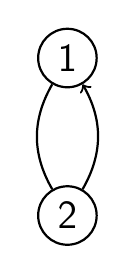
\begin{tikzpicture}[node distance=2cm, every loop/.style={},thick,main node/.style={circle,draw,font=\sffamily\Large}]
            \node[main node] (1) {1};
            \node[main node] (2) [below of=1] {2};
            \path[->] (2) edge[bend right] node {} (1);
            \path[-] (2) edge[bend left] node {} (1);
        \end{tikzpicture}
        \hspace{3cm}% NO SPACE!
        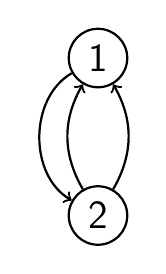
\begin{tikzpicture}[node distance=2cm, every loop/.style={},thick,main node/.style={circle,draw,font=\sffamily\Large}]
            \node[main node] (1) {1};
            \node[main node] (2) [below of=1] {2};
            \path[->] (2) edge[bend right] node {} (1);
            \path[->] (2) edge[bend left] node {} (1);
            \path[->] (1) edge[bend right=60] node {} (2);
        \end{tikzpicture}
    \end{center}

    Na esquerda temos um grafo misto, e na direita temos o mesmo grafo com sua aresta substituida por dois arcos em sentidos opostos. 

    Apesar da similaridade dos grafos, suas soluções para o problema do carteiro chinês diferem.
    \sloppy Uma solução ótima do problema para o primeiro grafo é $\{1, 2, 1\}$, enquanto que uma solução ótima possível para o segundo grafo é $\{1, 2, 1, 2, 1\}$, como representado visualmente a seguir.

    \begin{center}
        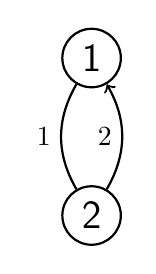
\begin{tikzpicture}[node distance=2cm, every loop/.style={},thick,main node/.style={circle,draw,font=\sffamily\Large}]
            \node[main node] (1) {1};
            \node[main node] (2) [below of=1] {2};
            \path[->] (2) edge[left, bend right] node {2} (1);
            \path[-] (2) edge[left, bend left] node {1} (1);
        \end{tikzpicture}
        \hspace{3cm}% NO SPACE!
        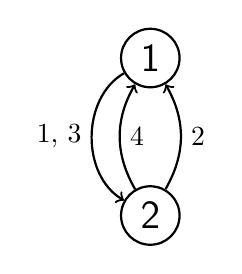
\begin{tikzpicture}[node distance=2cm, every loop/.style={},thick,main node/.style={circle,draw,font=\sffamily\Large}]
            \node[main node] (1) {1};
            \node[main node] (2) [below of=1] {2};
            \path[->] (2) edge[right, bend right] node {2} (1);
            \path[->] (2) edge[right, bend left] node {4} (1);
            \path[->] (1) edge[left, bend right=60] node {1, 3} (2);
        \end{tikzpicture}
    \end{center}

    Apesar de conseguirmos encontrar uma solução para o caso direcionado derivado, não há um modo trivial de transformar uma solução para tal caso em uma solução do caso não direcionado.

    Diferentemente do problema aplicado a grafos ou digrafos, o PCC aplicado a grafos mistos não possui solução polinomial, sendo um problema NP-difícil. 


    %%%%%%%%%%%%%% REF: PROBLEMA LINEAR DO KOEHLER E KAPPAUF
    %Uma solução para este caso proposta por Kappauf e Koehler\cite{mixed-pcc} que trataremos a seguir consiste em uma formulação do PCC como um problema linear inteiro.
    %%%%%%%%%%%%%%%%%%%%%%%%%%%%%%%%%%%%%%%%%%%

    %%%%%%%%%%%%%% REF: Paper do Frederickson, tem ao menos duas heuristicas pro misto ai: http://delivery.acm.org/10.1145/330000/322150/p538-frederickson.pdf?ip=195.176.178.182&id=322150&acc=ACTIVE%20SERVICE&key=FC66C24E42F07228%2E8FBBFD775A27C843%2E4D4702B0C3E38B35%2E4D4702B0C3E38B35&__acm__=1572510516_82601067be7298d3a7ff02d444c4cc9c

    Trataremos, portanto, de um algoritmo de aproximação para solucionar este problema, publicado em 1973 por Edmonds e Johnson \cite{edmonds-johnson} e posteriormente explicado em mais detalhes por Frederickson \cite{frederickson}. 

    O algoritmo é composto por três passos principais:

    \begin{enumerate}
        \item Adicionar cópias de arestas ao grafo de modo a tornar o grau de todo vértice par, considereando arcos como arestas sem orientação
        \item Igualar o grau de entrada e saída de todo vértice, adicionando cópias de arcos e orientando arestas existentes, mantendo par o grau de cada vértice
        \item Encontrar um circuito euleriano no digrafo construido
    \end{enumerate}
    

    Apresenta-se no algoritmo \ref{mixed-1} um pseudo-código adaptado de Frederickson \cite{frederickson} que segue esses passos.
    Seja $E$ o conjunto de arestas não direcionadas, $A$ o conjunto de arcos e $c$ a função de custo destas arestas e arcos.
    Tome $\delta(v)$ como a quantidade de arestas que incidem no vértice $v$, $\delta^+(v)$ como o grau de entrada de $v$, isto é, a quantidade de arcos que apontam a $v$ e $\delta^-(v)$ como o grau de saída de $v$, o número de arcos que saem de $v$.

    Definiremos como \textbf{grau total} de um vértice $v$, $\delta_t(v)$ a soma do grau de arestas não direcionadas, grau de entrada e saída, ou seja $\grt(v) = \gr(v) + \gre(v) + \grs(v)$.

    \begin{algorithm}
    \floatname{algorithm}{Algoritmo}%
    \caption{Função principal do algoritmo sugerido por Frederickson}
    \label{mixed-1}
    \begin{algorithmic}[1]
    \Function{Misto}{G, c} 
        \State $G' \gets $GRAU\_TOTAL\_PAR$(G, c)$ \Comment{Torna $\delta_t$ par}
        \State $M, U \gets $IGUALA\_GRAU\_DIR$(G', c)$ \Comment{Iguala $\delta^+$ e $\delta^-$}
        \State $M', U' \gets $GRAU\_PAR$(G', M, U)$ \Comment{Torna $\delta$ par, mantendo $\delta^+ = \delta^-$}
        \State $G_e = (V(G), U', M')$
        \State \Return CIRCUITO\_EULERIANO$(G_e)$ % TODO: Provar que tem como fazer esse circuito euleriano
    \EndFunction 
    \end{algorithmic}
    \end{algorithm}

    Para exemplificar o funcionamento do algoritmo, usaremos o seguinte grafo:

    \begin{figure}[H]
        \centering
        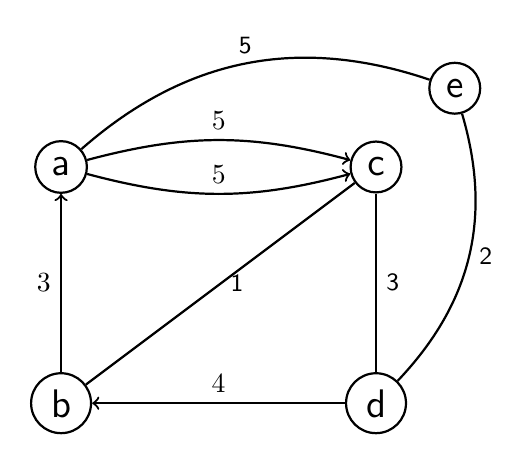
\begin{tikzpicture}[auto,node distance=3cm, every loop/.style={},thick,main node/.style={circle,draw,font=\sffamily\Large}]
            \node[main node] at (-3, 2) (a) {a};
            \node[main node] at (-3, -1) (b) {b};
            \node[main node] at (1, 2) (c) {c};
            \node[main node] at (1, -1) (d) {d};
            \node[main node] at (2, 3) (e) {e};

            \path[->] (a) edge[bend left=15] node [above] {5} (c);
            \path[->] (a) edge[bend right=15] node [above] {5} (c);
            \path[->] (b) edge[] node [left] {3} (a);
            \path[->] (d) edge[] node [above] {4} (b);

            \path[every node/.style={font=\sffamily\small}]
                (a) edge[bend left] node [above] {5} (e)
                (b) edge[] node [right] {1} (c)
                (c) edge node [right] {3} (d)
                (d) edge[bend right] node [right] {2} (e)
                ;
        \end{tikzpicture}
        \caption{Exemplo de grafo misto $G$}
        \label{mixed-exemplo}
    \end{figure}

    A função auxiliar ``GRAU\_TOTAL\_PAR'' apresentada no algoritmo \ref{mixed-grau-total-par} duplica arcos e arestas de $G$, criando um outro grafo $G'$ em que todos vértices possuem grau total par.

    Os arcos e arestas duplicados são escolhidos de modo a minimizar o custo total dos arcos e arestas de $G'$.
    
    \begin{algorithm}
    \floatname{algorithm}{Algoritmo}%
    \caption{Função auxiliar GRAU TOTAL PAR}
    \label{mixed-grau-total-par}
    \begin{algorithmic}[1]
    \Function{grau\_total\_par}{G,c}
        \State $(V, E, A) \gets G$
        \State $V' \gets \{v \in V : \delta_t(v)$ é impar$\}$
        \State $custMin \gets $ FLOYD\_WARSHALL$(G, c)$ 
            \Comment{Ignora o sentido dos arcos de $A$}
        \State $K \gets (V', V' \times V', custMin)$ 
            \Comment{Grafo completo de $V'$}
        \State $M \gets $ EMPARELHAMENTO\_PERFEITO\_MINIMO$(K)$
        \State Expande cada aresta de $M$ nos arcos e arestas do grafo original que ela representa, adicionando ao multiconjunto $A'$ os arcos expandidos e ao multiconjunto $E'$ as arestas expandidas.
        \State \Return $(V, E + E', A + A')$ 
    \EndFunction
    \end{algorithmic}
    \end{algorithm}

    \begin{figure}[H]
        \centering
        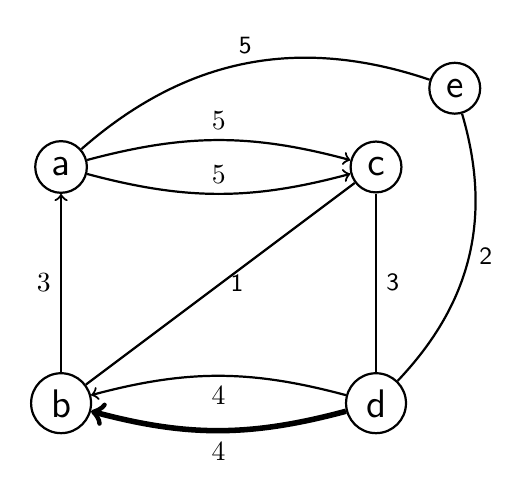
\begin{tikzpicture}[auto,node distance=3cm, every loop/.style={},thick,main node/.style={circle,draw,font=\sffamily\Large}]
            \node[main node] at (-3, 2) (a) {a};
            \node[main node] at (-3, -1) (b) {b};
            \node[main node] at (1, 2) (c) {c};
            \node[main node] at (1, -1) (d) {d};
            \node[main node] at (2, 3) (e) {e};

            \path[->] (a) edge[bend right=15] node [above] {5} (c);
            \path[->] (a) edge[bend left=15] node [above] {5} (c);
            \path[->] (b) edge[] node [left] {3} (a);
            \path[->] (d) edge[bend right=15] node [below] {4} (b);
            \path[->] (d) edge[line width=2,bend left=15] node [below] {4} (b);

            \path[every node/.style={font=\sffamily\small}]
                (a) edge[bend left] node [above] {5} (e)
                (b) edge[] node [right] {1} (c)
                (c) edge node [right] {3} (d)
                (d) edge[bend right] node [right] {2} (e)
                ;
        \end{tikzpicture}
        \caption{Em destaque o arco duplicado pela função \ref{mixed-grau-total-par}}
        \label{mixed-exemplo-grau-total}
    \end{figure}

    Por sua vez, a função ``IGUALA\_GRAU\_DIR'' devolve dois multiconjuntos $M$ e $U$, de arcos e arestas, respectivamente, de menor custo tal que todo vértice do grafo $(V, U, M)$ possui grau de entrada e saída iguais.

    O multiconjunto $M$ será formado por ao menos uma cópia de todos arcos de $A$ e cópias de arestas de $E$ direcionadas.
    Já $U$ será composto pelas arestas de $E$ que não foram direcionadas e adicionadas a $M$.

    \begin{algorithm}
    \floatname{algorithm}{Algoritmo}%
    \caption{Função auxiliar IGUALA GRAU DIR}
    \label{mixed-iguala-grau-dir}
    \begin{algorithmic}[1]
    \Function{iguala\_grau\_dir}{G, c, custMin}
    \State \Comment Devolve dois multiconjuntos $M$ e $U$, tal que $M$ contém ao menos uma cópia de cada arco de $A$ e algumas arestas de $E$ orientadas, e $U \subseteq E$ contém apenas arestas não orientadas e não pertencentes a $M$.
        \State $(V, E, A) \gets G$
        \For{$v \in V$}
            \State $b(v) \gets \delta^-(v) - \delta^+(v)$ \Comment Calcula a função demanda
        \EndFor
        \State $F \gets \{v \in V : b(v) < 0\}$
        \State $S \gets \{v \in V : b(v) > 0\}$
        \State $f \gets $ PROBLEMA\_DE\_TRANSPORTE$(F, S, custMin, b)$
        \State Seja $f_a$ a quantidade de fluxo que passa por cada arco $a \in A$ 
        \State Sejam $f_{uv}$ e $f_{vu}$ as quantidades de fluxo transportadas pelas duas orientações de uma aresta $uv \in E$

        \State $M, U \gets \emptyset$

        \For{$a \in A$}
            \State Insere $f_a + 1$ cópias do arco $a$ em $M$
        \EndFor
        \For{$uv \in E$}
            \If{$f_{vu} \geq 1$ ou $f_{uv} \geq 1$} \Comment{Se $custMin > 0$ é impossível que $f_{uv} \geq 1$ e $f_{vu} \geq 1$} ao mesmo tempo % TODO: PROVAR
                \State Insere $f_{uv}$ cópias de $uv$ e $f_{vu}$ cópias de $vu$ em $M$
            \Else 
                \State Insere $uv$ em $U$ 
            \EndIf
        \EndFor
        \State \Return $M, U$
    \EndFunction
    \end{algorithmic}
    \end{algorithm}

    \begin{figure}[H]
        \centering
        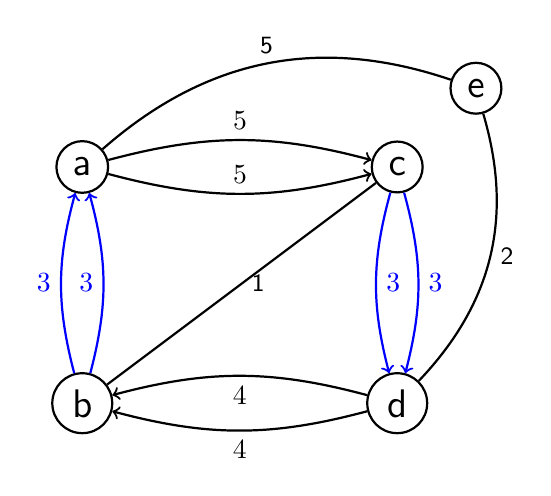
\begin{tikzpicture}[auto,node distance=3cm, every loop/.style={},thick,main node/.style={circle,draw,font=\sffamily\Large}]
            \node[main node] at (-3, 2) (a) {a};
            \node[main node] at (-3, -1) (b) {b};
            \node[main node] at (1, 2) (c) {c};
            \node[main node] at (1, -1) (d) {d};
            \node[main node] at (2, 3) (e) {e};

            \path[->] (a) edge[bend right=15] node [above] {5} (c);
            \path[->] (a) edge[bend left=15] node [above] {5} (c);
            \path[->] (b) edge[blue, bend right=15] node [left] {3} (a);
            \path[->] (b) edge[blue, bend left=15] node [left] {3} (a);
            \path[->] (d) edge[bend right=15] node [below] {4} (b);
            \path[->] (d) edge[bend left=15] node [below] {4} (b);
            \path[->] (c) edge[blue, bend right=15] node [right] {3} (d);
            \path[->] (c) edge[blue, bend left=15] node [right] {3} (d);

            \path[every node/.style={font=\sffamily\small}]
                (a) edge[bend left] node [above] {5} (e)
                (b) edge[] node [right] {1} (c)
                (d) edge[bend right] node [right] {2} (e)
                ;
        \end{tikzpicture}
        \caption{O arco $ba$ e a aresta orientada $cd$ duplicados pela função \ref{mixed-iguala-grau-dir}}
        \label{mixed-exemplo-grau-dir}
    \end{figure}

    Apesar do algoritmo \ref{mixed-iguala-grau-dir} devolver multiconjuntos $M, U$ que igualam o grau de entrada e saída dos vértices de $V$, ele não garante que o grau total desses vértices continua par, como pode-se notar no exemplo da figura \ref{mixed-exemplo-grau-dir}.
    Por esse motivo é necessária a função GRAU PAR, do algoritmo \ref{mixed-grau-par}, que deriva de $M, U$ outros multiconjuntos $M'$ e $U'$ que tornam $\delta_t$ par, mantêm a igualdade de $\delta^+$ e $\delta^-$ e por consequência, tornam $\gr$ par para todo vértice.

    \begin{algorithm}
    \floatname{algorithm}{Algoritmo}%
    \caption{Função auxiliar GRAU PAR}
    \label{mixed-grau-par}
    \begin{algorithmic}[1]
        \Function{grau\_par}{G, M, U}
            %\State \Comment{Devolve os multiconjuntos $M'$, $U'$, que mantêm, para todo vértice, a igualdade dos graus $\delta^+$ e $\delta^-$ e torna $\delta^+ + \delta^- + \delta$ par.}
            \State $U' \gets U$
            \State O multiconjunto $M' \subseteq M$ deverá possuir apenas as arestas direcionadas e as cópias de arcos criadas em $GRAU\_DIR$.
            \State Seja $V' = \{v \in V : \delta^+ + \delta^- + \delta$ é ímpar $\}$

            \While{$V'$ não é vazio}
                \State Seleciona um vértice qualquer $v_{ini}$ de $V'$ 
                \State $v \gets v_{ini}$
                \While{$v \in V'$}
                    \State $V' \gets V' \setminus v$
                    \Repeat 
                        \State Seja $a$ um arco incidente a $v$, da forma $vw$ ou $wv$, pertencente a $M'$
                        \If{$a$ é o arco $vw$}
                            \State Insere outra cópia de $a$ em $M'$ \label{alg:duplica}
                        \Else
                            \State Apague uma cópia de $a$ de $M'$ \label{alg:deleta}
                        \EndIf
                        \State $v \gets w$
                    \Until{$v \notin V'$}
                    \Repeat
                        \State Remove uma aresta $vw$ de $U'$
                        \State Orienta tal aresta no sentido de $v$ para $w$ e a adiciona em $M'$ \label{alg:orienta}
                        \State $v \gets w$
                    \Until{$v \notin V'$ e $v \neq v_{ini}$}
                \EndWhile
            \EndWhile
        \EndFunction
    \end{algorithmic}
    \end{algorithm}

    \begin{figure}[H]
        \centering
        \begin{minipage}{.5\textwidth}
          \centering
            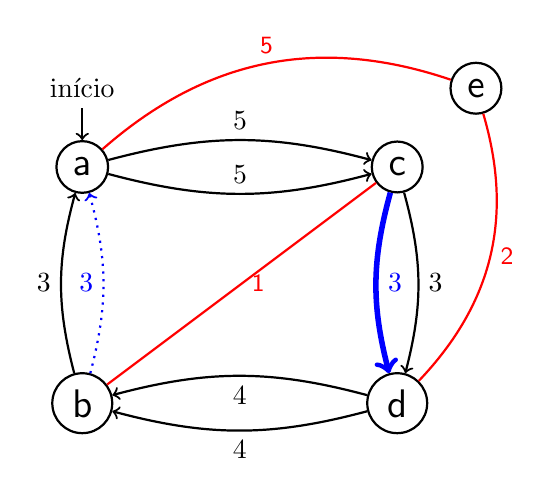
\begin{tikzpicture}[auto,node distance=3cm, every loop/.style={},thick,main node/.style={circle,draw,font=\sffamily\Large}]
                \node[main node] at (-3, 2) (a) {a};
                \node[main node] at (-3, -1) (b) {b};
                \node[main node] at (1, 2) (c) {c};
                \node[main node] at (1, -1) (d) {d};
                \node[main node] at (2, 3) (e) {e};
                \node[] at (-3, 3) (ini) {início};

                \path[->] (ini) edge[] node {} (a);

                \path[->] (a) edge[bend right=15] node [above] {5} (c);
                \path[->] (a) edge[bend left=15] node [above] {5} (c);
                \path[->] (b) edge[dotted, blue, bend right=15] node [left] {3} (a);
                \path[->] (b) edge[bend left=15] node [left] {3} (a);
                \path[->] (d) edge[bend right=15] node [below] {4} (b);
                \path[->] (d) edge[bend left=15] node [below] {4} (b);
                \path[->] (c) edge[line width=2, blue, bend right=15] node [right] {3} (d);
                \path[->] (c) edge[bend left=15] node [right] {3} (d);

                \path[every node/.style={font=\sffamily\small}]
                    (a) edge[red, bend left] node [above] {5} (e)
                    (b) edge[red] node [right] {1} (c)
                    (d) edge[red, bend right] node [right] {2} (e)
                    ;
            \end{tikzpicture}
          \label{exmixed1}
        \end{minipage}%
        \begin{minipage}{.5\textwidth}
          \centering
            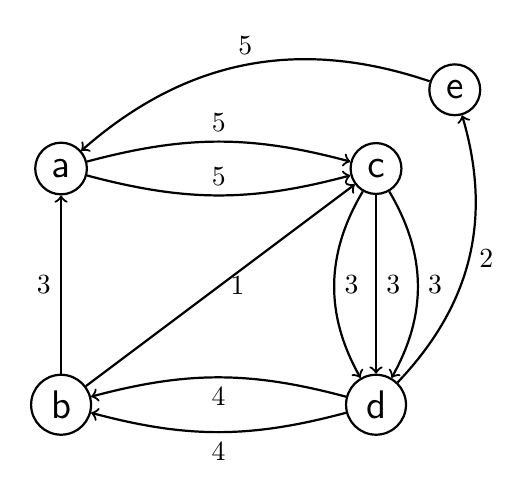
\begin{tikzpicture}[auto,node distance=3cm, every loop/.style={},thick,main node/.style={circle,draw,font=\sffamily\Large}]
                \node[main node] at (-3, 2) (a) {a};
                \node[main node] at (-3, -1) (b) {b};
                \node[main node] at (1, 2) (c) {c};
                \node[main node] at (1, -1) (d) {d};
                \node[main node] at (2, 3) (e) {e};

                \path[->] (a) edge[bend right=15] node [above] {5} (c);
                \path[->] (a) edge[bend left=15] node [above] {5} (c);
                \path[->] (b) edge[] node [left] {3} (a);
                \path[->] (d) edge[bend right=15] node [below] {4} (b);
                \path[->] (d) edge[bend left=15] node [below] {4} (b);
                \path[->] (c) edge[bend right] node [right] {3} (d);
                \path[->] (c) edge[] node [right] {3} (d);
                \path[->] (c) edge[bend left] node [right] {3} (d);
                \path[->] (b) edge[] node [right] {1} (c);
                \path[->] (d) edge[bend right] node [right] {2} (e);
                \path[->] (e) edge[bend right] node [above] {5} (a);
            \end{tikzpicture}
          \label{exmixed2}
        \end{minipage}%
        \caption{Criação de $M', U'$, a partir de $M, U$ pelo algoritmo \ref{mixed-grau-par}}
        \label{ex-grau-par}
    \end{figure}

    No exemplo \ref{ex-grau-par} o algoritmo \ref{mixed-grau-par} toma o circuito $\{a, b, c, d, e, a\}$ para realizar a construção de $M', U'$. 
    Em azul destacam-se os arcos de $M$ e em vermelho as arestas de $U$ escolhidos.

    Como o arco $ab$ é percorrido pelo circuito no sentido contrário, o mesmo é deletado do conjunto $M'$ (linha \ref{alg:deleta}), já o arco $cd$, percorrido no sentido correto, é duplicado (linha \ref{alg:duplica}).
    As arestas do circuito são todas orientadas no sentido em que são percorridas: $bc, de, ea$ (linha \ref{alg:orienta}).

    Deste modo conseguem-se multiconjuntos $M', U'$ de mesmo custo que $M, U$ e que mantêm $\gre = \grs$ e $\gr$ par para todo vértice de $G$.

    \begin{theorem} 
        Um grafo misto fortemente conexo que possui $\delta(v)$ par e $\delta^+(v) = \delta^-(v)$ para todo vértice $v$, possui um circuito euleriano.
        \label{mixed-eulerian}
    \end{theorem}

    \begin{proof}
        Seja $G = (V, E, A)$, sendo $E$ um multiconjunto de arestas e $A$ um multiconjunto de arcos.
        Definimos como $G_e$ o grafo induzido pelas arestas de $E$, e de $G_a$ o grafo induzido por $A$.
        Apesar de não necessariamente conexos, ainda valerá que todo vértice de $G_e$ possui um $\delta$ par e que todo vértice de $G_a$ tem $\gre = \grs$.
        
        $G_e$ será composto por diferentes componentes conexas com vértices de grau par, consequentemente cada componente será euleriana, pelo teorema \ref{euler}.
        Sejam $C_1, C_2, \dots, C_k$  os circuitos eulerianos das $k$ componentes de $G_e$.

        A mesma análise pode ser feita com o grafo $G_a$, cada uma de suas componentes fortemente conexas possuirá grau de entrada e saída iguais, sendo assim grafos eulerianos pelo teorema \ref{euler-digraph}. 
        Sejam $C'_1, \dots, C'_l$ os circuitos eulerianos dessas componenetes.

        Pode-se definir um procedimento de união de dois circuitos em um único circuito se ambos possuem ao menos um vértice em comum:
        
        Digamos que dois circuitos $\mathcal{C}_i$ e $\mathcal{C}_j$ possuem um vértice $v$ em comum.
        Podemos descrever ambos circuitos por seus arcos ou arestas do seguinte modo:

        \[
            \mathcal{C}_i = \{ vw_1, w_1w_2, \dots, w_nv \}
        \]
        \[
            \mathcal{C}_j = \{ vu_1, u_1u_2, \dots, u_mv \}
        \]

        Se representados desse modo, a união dos circuitos será equivalente à justaposição de ambos:

        \[
            \mathcal{C}_i \cup \mathcal{C}_j = \{ vw_1, w_1w_2, \dots w_nv, vu_1, u_1u_2, \dots, u_mv \}
        \]
        
        A união de todos circuitos $C_1, \dots C_k$ e $C'_1, \dots, C'_l$ forma um circuito euleriano do grafo original $G$.

        Como o grafo original é fortemente conexo, sempre é possível realizar a união de todos circuitos.
    Do contrário, se não houver meio de realizar tal união deverá existir um circuito $C_i$ que não possui vértice em comum com nenhum outro circuito, implicando assim que $\bigcup \mathcal{C}_i = G$ não seria fortemente conexo, contradizendo a base do raciocínio.
    \end{proof}

    Como o exemplo apresentado é transformado em um digrafo euleriano após a execução de \ref{mixed-grau-par}, basta tomar o circuito euleriano do mesmo para derivar uma solução do grafo misto original, como mostrado na figura \ref{fig:mixed-ex-sol}.


    \begin{figure}
        \begin{minipage}{.5\textwidth}
          \centering
            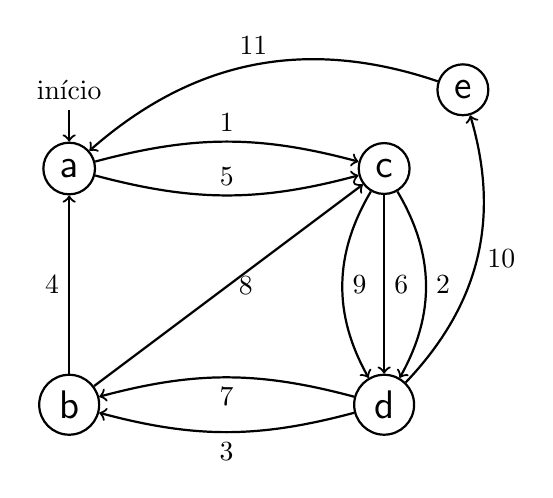
\begin{tikzpicture}[auto,node distance=3cm, every loop/.style={},thick,main node/.style={circle,draw,font=\sffamily\Large}]
                \node[main node] at (-3, 2) (a) {a};
                \node[main node] at (-3, -1) (b) {b};
                \node[main node] at (1, 2) (c) {c};
                \node[main node] at (1, -1) (d) {d};
                \node[main node] at (2, 3) (e) {e};
                \node[] at (-3, 3) (ini) {início};
                \path[->] (ini) edge[] node [] {} (a);

                \path[->] (a) edge[bend right=15] node [above] {5} (c);
                \path[->] (a) edge[bend left=15] node [above] {1} (c);
                \path[->] (b) edge[] node [left] {4} (a);
                \path[->] (d) edge[bend right=15] node [below] {7} (b);
                \path[->] (d) edge[bend left=15] node [below] {3} (b);
                \path[->] (c) edge[bend right] node [right] {9} (d);
                \path[->] (c) edge[] node [right] {6} (d);
                \path[->] (c) edge[bend left] node [right] {2} (d);
                \path[->] (b) edge[] node [right] {8} (c);
                \path[->] (d) edge[bend right] node [right] {10} (e);
                \path[->] (e) edge[bend right] node [above] {11} (a);
            \end{tikzpicture}
        \end{minipage}%
        \begin{minipage}{.5\textwidth}
            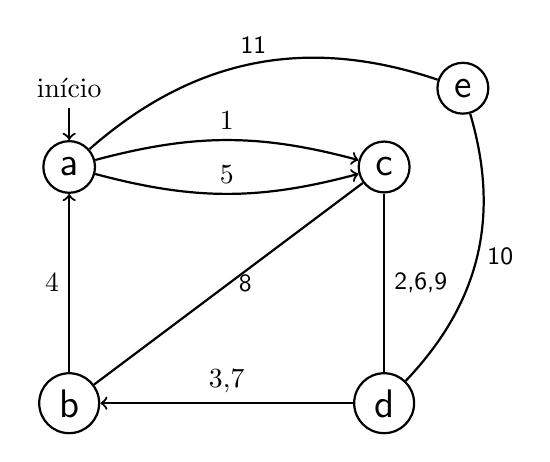
\begin{tikzpicture}[auto,node distance=3cm, every loop/.style={},thick,main node/.style={circle,draw,font=\sffamily\Large}]
                \node[main node] at (-3, 2) (a) {a};
                \node[main node] at (-3, -1) (b) {b};
                \node[main node] at (1, 2) (c) {c};
                \node[main node] at (1, -1) (d) {d};
                \node[main node] at (2, 3) (e) {e};
                \node[] at (-3, 3) (ini) {início};
                \path[->] (ini) edge[] node [] {} (a);

                \path[->] (a) edge[bend left=15] node [above] {1} (c);
                \path[->] (a) edge[bend right=15] node [above] {5} (c);
                \path[->] (b) edge[] node [left] {4} (a);
                \path[->] (d) edge[] node [above] {3,7} (b);

                \path[every node/.style={font=\sffamily\small}]
                    (a) edge[bend left] node [above] {11} (e)
                    (b) edge[] node [right] {8} (c)
                    (c) edge node [right] {2,6,9} (d)
                    (d) edge[bend right] node [right] {10} (e)
                    ;
            \end{tikzpicture}
        \end{minipage}
        \caption{Circuito euleriano de $G_e$ e solução do PCC de $G$, respectivamente}
        \label{fig:mixed-ex-sol}
    \end{figure}

    \begin{lemma}
        \label{mixed-custo-igual}
        Seja $C(M,U)$ o custo dos multiconjuntos $M,U$, ou seja, a soma do custo dos arcos e arestas que compõem $M$ e $U$.

        Vale que $C(M', U') = C(M, U)$. 
        Isto é, os multiconjuntos $M', U'$ retornados pela função \ref{mixed-grau-par} possuem o mesmo custo que os multiconjuntos $M, U$, retornados por \ref{mixed-iguala-grau-dir}.
    \end{lemma}

    \begin{proof}
        Como os conjuntos $M, U$ foram gerados resolvendo um problema de transporte, possuimos a garantia que eles são os multiconjuntos de menor custo que igualam o grau de entrada e saída de todos vértices de um grafo $G(V, A, E)$. 
        Em particular, vale que $C(M', U') \geq C(M, U)$. 

        Para mostrar que $C(M', U') = C(M, U)$ chegaremos a uma contradição assumindo que $C(M', U') > C(M, U)$:

        Os multiconjuntos $M'$ e $U'$ são construidos pelo algoritmo \ref{mixed-grau-par} a partir de $M$ e $U$. 
        Como exemplificado na figura \ref{ex-grau-par} na construção de $M', U'$ podem ocorrer três tipos de eventos:

        \begin{enumerate}
            \item Um arco $a \in M$ é duplicado em $M'$
            \item Um arco $a \in M$ é deletado em $M'$
            \item Uma aresta $e \in U$ é orientada e adicionada a $M'$
        \end{enumerate}
        
        Dos três tipos de eventos listados, apenas os dois primeiros mudam o custo dos multiconjuntos $M', U'$ em relação a $M, U$.
        Um evento do tipo 1 aumenta o custo de $M', U'$ pelo valor do custo de $a$, assim como um evento do tipo 2 diminui o custo de $M', U'$ pelo custo de $a$, em relação ao custo de $M, U$.

        Sendo assim, podemos definir $C(M', U')$ como $C(M', U') = C(M, U) + C_+ - C_-$, sendo $C_+$ a soma do custo dos arcos duplicados (evento 1) e $C_-$ a soma do custo dos arcos deletados no algoritmo (evento 2).

        Se $C(M', U') > C(M, U)$, como assumimos, vale que:

        \begin{align*}
            C(M, U) + C_+ - C_- &= C(M', U') \\
            C_+ - C_- &= C(M', U') - C(M, U) \\
            C_+ - C_- &> 0 \\ 
        \end{align*}

        Vamos tomar agora outros multiconjuntos $M'', U''$, em que $U'' = U'$ e que $M''$ será definido a partir de $M$ com três eventos, de modo análogo a $M'$:
        
        \begin{enumerate}
            \item Se um arco $a \in M$ foi duplicado em $M'$, o mesmo será deletado de $M''$.
            \item Se um arco $a \in M$ foi deletado em $M'$, o mesmo será duplicado em $M''$.
            \item Se uma aresta $e \in U$ foi orientada da forma $uv$ e adicionada a $M'$, a mesma será adicionada a $M''$ com a orientação oposta: $vu$.
        \end{enumerate}

        Para exemplificar essa definição, na figura \ref{fig:mixed-ex-lema} comparam-se os conjuntos $M', U'$ e $M'', U''$ do exemplo tratado nesta seção.

        \begin{figure}[H]
            \centering
            \begin{minipage}{.5\textwidth}
              \centering
                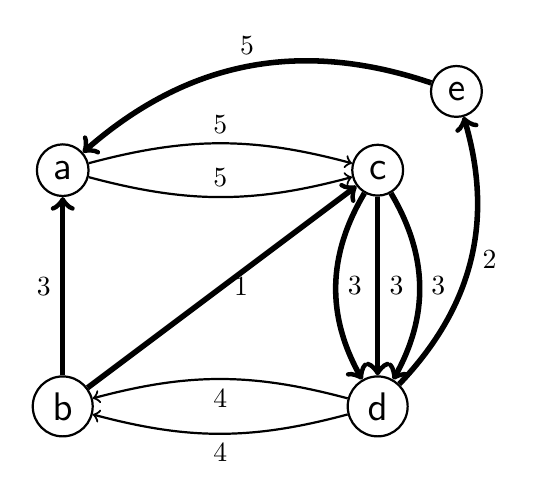
\begin{tikzpicture}[auto,node distance=3cm, every loop/.style={},thick,main node/.style={circle,draw,font=\sffamily\Large}]
                    \node[main node] at (-3, 2) (a) {a};
                    \node[main node] at (-3, -1) (b) {b};
                    \node[main node] at (1, 2) (c) {c};
                    \node[main node] at (1, -1) (d) {d};
                    \node[main node] at (2, 3) (e) {e};

                    \path[->] (a) edge[bend right=15] node [above] {5} (c);
                    \path[->] (a) edge[bend left=15] node [above] {5} (c);
                    \path[->] (b) edge[line width=2] node [left] {3} (a);
                    \path[->] (d) edge[bend right=15] node [below] {4} (b);
                    \path[->] (d) edge[bend left=15] node [below] {4} (b);
                    \path[->] (c) edge[line width=2, bend right] node [right] {3} (d);
                    \path[->] (c) edge[line width=2] node [right] {3} (d);
                    \path[->] (c) edge[line width=2, bend left] node [right] {3} (d);
                    \path[->] (b) edge[line width=2] node [right] {1} (c);
                    \path[->] (d) edge[line width=2, bend right] node [right] {2} (e);
                    \path[->] (e) edge[line width=2, bend right] node [above] {5} (a);
                \end{tikzpicture}
            \end{minipage}%
            \begin{minipage}{.5\textwidth}
              \centering
                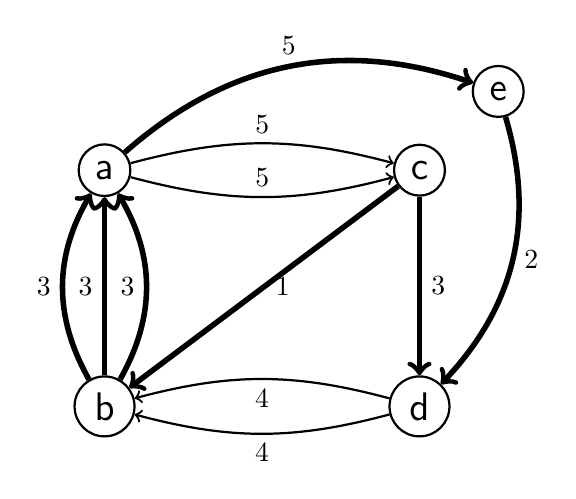
\begin{tikzpicture}[auto,node distance=3cm, every loop/.style={},thick,main node/.style={circle,draw,font=\sffamily\Large}]
                    \node[main node] at (-3, 2) (a) {a};
                    \node[main node] at (-3, -1) (b) {b};
                    \node[main node] at (1, 2) (c) {c};
                    \node[main node] at (1, -1) (d) {d};
                    \node[main node] at (2, 3) (e) {e};

                    \path[->] (a) edge[bend right=15] node [above] {5} (c);
                    \path[->] (a) edge[bend left=15] node [above] {5} (c);
                    \path[->] (b) edge[line width=2, bend right] node [left] {3} (a);
                    \path[->] (b) edge[line width=2, bend left] node [left] {3} (a);
                    \path[->] (b) edge[line width=2] node [left] {3} (a);
                    \path[->] (d) edge[bend right=15] node [below] {4} (b);
                    \path[->] (d) edge[bend left=15] node [below] {4} (b);
                    \path[->] (c) edge[line width=2] node [right] {3} (d);
                    \path[->] (c) edge[line width=2] node [right] {1} (b);
                    \path[->] (e) edge[line width=2, bend left] node [right] {2} (d);
                    \path[->] (a) edge[line width=2, bend left] node [above] {5} (e);
                \end{tikzpicture}
            \end{minipage}%
            \caption{ Diferenças entre $M', U'$ e $M'', U''$, respectivamente}
            \label{fig:mixed-ex-lema}
        \end{figure}

        Como $M'', U''$ também igualam os graus de entrada e saída de $G$, então vale que $C(M'', U'') \geq C(M, U)$.
        Além disso, podemos definir tal custo como $C(M'', U'') = C(M, U) + C_- - C_+$.
        
        Sendo assim:

        \begin{align*}
            C(M, U) + C_- - C_+ &= C(M'', U'') \\
            C_+ - C_- &= C(M, U) - C(M'', U'') \\
            C_+ - C_- &\leq 0 
        \end{align*}

        Como haviamos provado anteriormente que $C_+ - C_- > 0$, chegamos a uma contradição.
        Provando por absurdo, que $C(M', U') = C(M, U)$.
    \end{proof}

    \begin{theorem}{\cite{frederickson}}
        Seja $C$ o custo de uma solução ótima do problema do carteiro chinês em um grafo misto $G$, e $C'$ o custo da solução construída pelo algoritmo descrito, vale que:
        \[
            C'/C \leq 2
        \]
    \end{theorem}

    \begin{proof}
        Assume-se que todas arestas e arcos de $G$ tenham um custo positivo. 

        Seja $G^*$ o grafo $G$ com todos arcos e arestas duplicadas e $C^*$ o custo da solução dada pelo algoritmo MISTO ao grafo $G^*$.

        Como o grau total de todos vértices de $G^*$ é par, as únicas funções que modificarão o grafo $G^*$ do algoritmo serão \ref{mixed-iguala-grau-dir} e \ref{mixed-grau-par}.
        Além disso, como a função \ref{mixed-iguala-grau-dir} encontra multiconjuntos de arcos e arestas que igualam os graus de entrada e saída de $G^*$ com o menor custo possível (solucionando o problema de transporte modelado) e como a função \ref{mixed-grau-par} modifica os multiconjuntos sem modificar o seu custo (lema \ref{mixed-custo-igual}), podemos dizer que $C^*$ é o custo ótimo para a solução do PCC para o grafo misto $G^*$. 

        Sendo assim, como a solução ótima de $G$, de custo $C$, pode ser duplicada para encontrar uma solução de $G^*$ também deve valer que $C^* \leq 2C$.

        Definimos agora $G'$ como o grafo retornado pela função \ref{mixed-grau-total-par} com parâmetro $G$.
        A função \ref{mixed-grau-total-par} constrói $G'$ duplicando arcos e arestas de caminhos entre vértices de grau total ímpar de $G$, minimizando o custo de tal construção.

        Pode-se afirmar que não existirá em $G'$ um arco ou aresta $uv$ que foi duplicado mais que uma vez na função \ref{mixed-grau-total-par}, pois se existisse poderia-se remover de $G'$ duas cópias de $uv$ que conseguiria-se outro grafo com mesma paridade total de vértices e custo menor.

        Assim, como cada aresta e arco de $G$ é duplicado no máximo uma vez em $G'$, podemos afirmar que os multiconjuntos de arcos e arestas de $G'$ estarão contidos nos multiconjuntos de $G^*$ e por isso, o custo $C'$ da solução dada pelo algoritmo MISTO ao grafo $G$ deverá ser menor ou igual a $C^*$.
        
        \begin{align*}
            C' \leq C^* &\leq 2C \\
            C'/C &\leq 2
        \end{align*}

        Provando assim que o algoritmo MISTO é uma 2-aproximação para o problema do carteiro misto.
    \end{proof}

    \subsection{Problema do carteiro rural}
    % Ref https://core.ac.uk/download/pdf/37350985.pdf
    
    Nesta variação, além do grafo $G(V, A)$, sendo $V$ o conjunto de vértices e $A$ o conjunto de arestas, uma função de custo $c_e$, para algum $e\in A$, é também necessário se especificar um subconjunto $R \subseteq A$. 

    Nesta versão mais geral do PCC devemos realizar o planejamento de uma rota de custo mínimo que se inicia e termina no mesmo vértice e passa ao menos uma vez por toda aresta pertencente a $R$. 
    Isto é, não há necessidade de se percorrer as arestas de $A \setminus R$.

    Denomina-se esta variação de Problema do Carteiro Rural (PCR).

    Esse problema possui aplicações mais gerais que a sua versão original, por exemplo: pode-se modelar a rota de um carteiro que não necessariamente precisa percorrer todas as ruas de uma cidade, ou mesmo a rota de um ônibus escolar, que precisa passar apenas nas ruas dos alunos que ele atende, e não necessariamente por todas ruas de um bairro.

    O PCR é um problema NP-completo \cite{rural-np-complete}. %e np dificil

    De modo similar aos outros casos do PCC, a solução padrão para este problema consiste em estender $G$ adicionando cópias de arestas de modo que o mesmo se torne euleriano e em sequência construir uma solução a partir do circuito euleriano do grafo estendido.

    Para realizar a primeira parte da solução do problema, ou seja, criar uma extensão euleriana de $G$, serão apresentadas tanto heurísticas quanto discussões das soluções ótimas existentes.

        \subsubsection{PCR em grafos não direcionados}


        \textbf{Heurística da árvore geradora mínima}

        Em 1979 Christofides sugeriu um algoritmo aproximado para o problema do caixeiro viajante que possui o melhor fator de aproximação para grafos gerais provado \cite{wiki-christofides}. % https://en.wikipedia.org/wiki/Christofides_algorithm

        Será apresentada uma adaptação de tal algoritmo que pode ser aplicada ao PCR, sugerida por Frederickson (1979).
        Pode-se provar que tal algoritmo possui uma razão de aproximação de $3/2$ para grafos cuja função de custo respeita a desigualdade triangular. 

        Para resolver o PCR em grafos não direcionados define-se um grafo $G' = (V', A')$, onde $V' = \{ u \in V : (u, v) \in R$ para algum $v \in V\}$.

        $A'$ é obtido por adicionar ao conjunto $A$ uma aresta $(v_i, v_j)$ para todo par $v_i, v_j \in V'$ cujo custo é igual ao custo do menor caminho de $v_i$ a $v_j$; e retirar-se de $A'$ duplicatas de arestas paralelas de mesmo custo e todas arestas $(u, v) \in A \setminus R$ tal que $c_{uv} = c_{uw} + c_{wv}$ para algum vértice $w$.

        Pode-se visualizar um exemplo de tal separação a seguir:


        \begin{figure}[H]
            \centering
            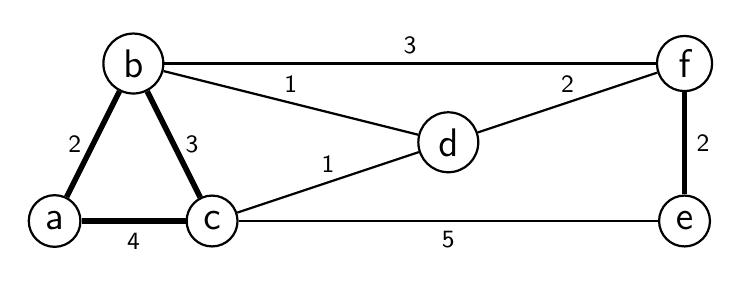
\begin{tikzpicture}[auto,node distance=3cm, every loop/.style={},thick,main node/.style={circle,draw,font=\sffamily\Large}]
                \node[main node] at (-5, -1) (a) {a};
                \node[main node] at (-4, 1) (b) {b};
                \node[main node] at (-3, -1) (c) {c};
                \node[main node] at (0, 0) (d) {d};
                \node[main node] at (3, -1) (e) {e};
                \node[main node] at (3, 1) (f) {f};

                \path[every node/.style={font=\sffamily\small}]
                    (a) edge[line width=2] node [left] {2} (b)
                    (b) edge[line width=2] node [right] {3} (c)
                    (a) edge[line width=2] node [below] {4} (c)
                    (b) edge node [above] {1} (d)
                    (b) edge node [above] {3} (f)
                    (c) edge node [above] {1} (d)
                    (c) edge node [below] {5} (e)
                    (d) edge node [above] {2} (f)
                    (e) edge[line width=2] node [right] {2} (f)
                    ;
            \end{tikzpicture}
            \caption{Exemplo de grafo $G$, destacam-se no mesmo as arestas pertencentes a $R$}
            \label{grafo-original}
        \end{figure}

        Define-se o conjunto de vértices de $G'$: $V' = \{a, b, c, e, f\}$.
        Exclui-se de tal conjunto apenas o vértice $d$, que não possui qualquer ligação com aresta em $R$.

    O conjunto $A'$ é definido em duas etapas: primeiramente criam-se novas arestas entre os vértices de $V'$ com custo igual ao custo da menor distância entre os mesmos vértices em $G$, tais arestas são representadas em azul na imagem \ref{grafo-intermediario}.


        \begin{figure}[H]
            \centering
            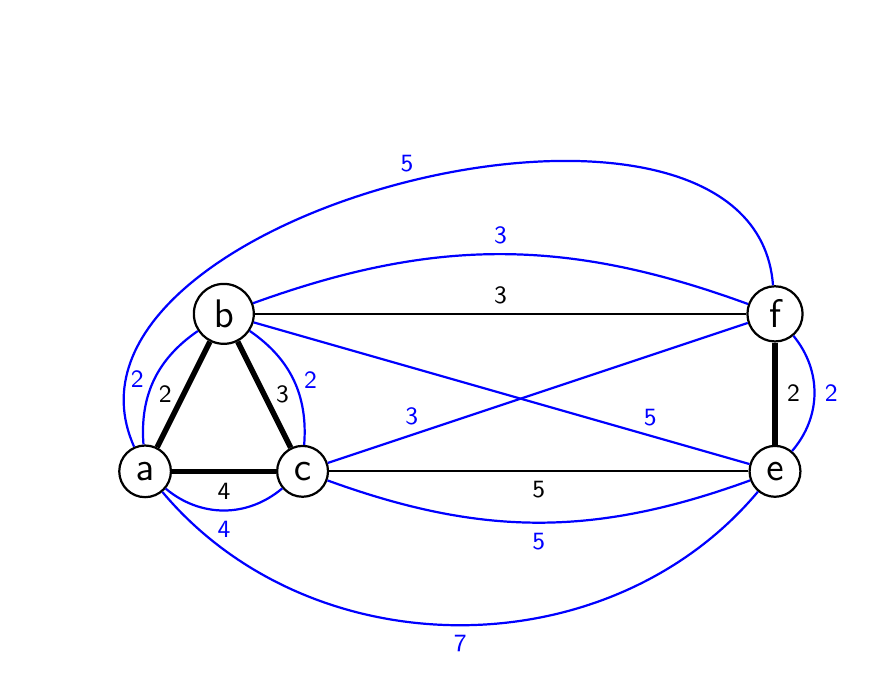
\begin{tikzpicture}[auto,node distance=3cm, every loop/.style={},thick,main node/.style={circle,draw,font=\sffamily\Large}]
                \node[main node] at (-5, -1) (a) {a};
                \node[main node] at (-4, 1) (b) {b};
                \node[main node] at (-3, -1) (c) {c};
                \node[main node] at (3, -1) (e) {e};
                \node[main node] at (3, 1) (f) {f};

                \path[every node/.style={font=\sffamily\small}]
                    (a) edge[line width=2] node [left] {2} (b)
                    (a) edge[blue, bend left] node [left] {2} (b)
                    (b) edge[line width=2] node [right] {3} (c)
                    (b) edge[blue, bend left] node [right] {2} (c)
                    (a) edge[line width=2] node [below] {4} (c)
                    (a) edge[blue, bend right=40] node [below] {4} (c)
                    (b) edge node [above] {3} (f)
                    (b) edge[blue, bend left=20] node [above] {3} (f)
                    (c) edge node [below] {5} (e)
                    (c) edge[blue, bend right=20] node [below] {5} (e)
                    (e) edge[line width=2] node [right] {2} (f)
                    (e) edge[blue, bend right=40] node [right] {2} (f)
                    (c) edge[blue] node [above, pos=0.2] {3} (f)
                    (e) edge[blue] node[above, pos=0.2] {5} (b)
                    (f) edge[blue, bend right=100] node[above] {5} (a)
                    (e) edge[blue, bend left=50] node[below] {7} (a)
                    ;
            \end{tikzpicture}
            \caption{Grafo intermediário na transformação de $G$ em $G'$}
            \label{grafo-intermediario}
        \end{figure}


        Após a criação das novas arestas são deletadas do grafo todas arestas $uv \notin R$ tal que existe $w \in V'$ para que $c_{uv} = c_{uw} + c_{wv}$, assim como as arestas paralelas não pertencentes a $R$ de mesmo custo.
        % CONFERIR PQ TA DIFERENTE DO PAPER

        No exemplo são retiradas de $A'$ uma cópia das arestas $ab, ac, bf, ce, ef$ pois já existem arestas paralelas a estas de mesmo custo.
        Retiram-se também as arestas: $af$ já que $c_{af} = c_{ab} + c_{bf}$, $be$ já que $c_{be} = c_{bf} + c_{fe}$, $ae$ já que $c_{ae} = c_{af} + c_{fe}$.


        \begin{figure}[H]
            \centering
            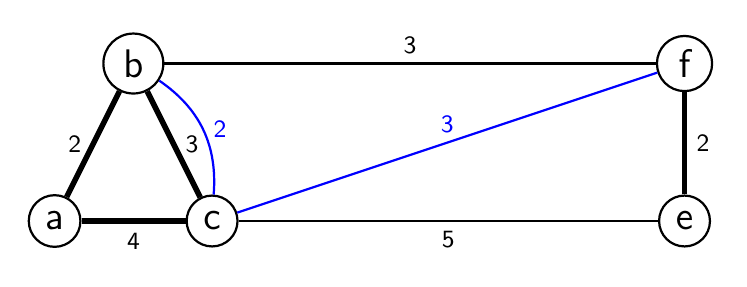
\begin{tikzpicture}[auto,node distance=3cm, every loop/.style={},thick,main node/.style={circle,draw,font=\sffamily\Large}]
                \node[main node] at (-5, -1) (a) {a};
                \node[main node] at (-4, 1) (b) {b};
                \node[main node] at (-3, -1) (c) {c};
                \node[main node] at (3, -1) (e) {e};
                \node[main node] at (3, 1) (f) {f};

                \path[every node/.style={font=\sffamily\small}]
                    (a) edge[line width=2] node [left] {2} (b)
                    (b) edge[line width=2] node [right] {3} (c)
                    (b) edge[blue, bend left] node [right] {2} (c)
                    (a) edge[line width=2] node [below] {4} (c)
                    (b) edge node [above] {3} (f)
                    (c) edge node [below] {5} (e)
                    (e) edge[line width=2] node [right] {2} (f)
                    (c) edge[blue] node [above] {3} (f)
                    ;
            \end{tikzpicture}
            \caption{Grafo transformado $G'$}
            \label{grafo-transformado}
        \end{figure}
        
        Considere o subgrafo de $G'$ induzido pelas arestas de $R$. Este grafo possui $k$ componentes conexas, que são denominadas $G_1, G_2, \dots, G_k$. 

        No exemplo tal separação gera dois subgrafos $G_1$ e $G_2$, que são representadas na figura \ref{r-separacao}, compostas pelos conjuntos de vértices $V_1 = \{a, b, c\}$ e $V_2 = \{f, e\}$ respectivamente.

        \begin{figure}[H]
            \centering
            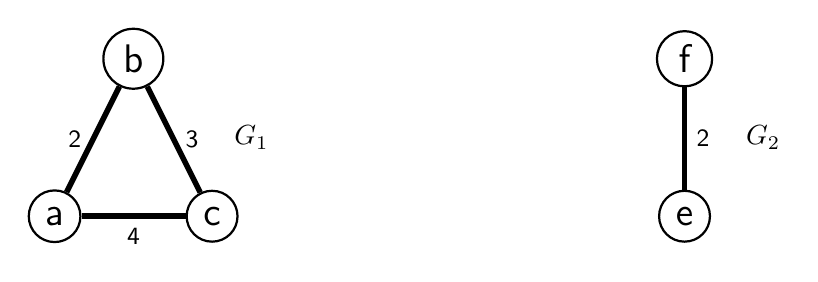
\begin{tikzpicture}[auto,node distance=3cm, every loop/.style={},thick,main node/.style={circle,draw,font=\sffamily\Large}]
                \node[main node] at (-5, -1) (a) {a};
                \node[main node] at (-4, 1) (b) {b};
                \node[main node] at (-3, -1) (c) {c};
                \node[main node] at (3, -1) (e) {e};
                \node[main node] at (3, 1) (f) {f};
                \node[] at (-2.5, 0) (g1) {$G_1$};
                \node[] at (4, 0) (g2) {$G_2$};

                \path[every node/.style={font=\sffamily\small}]
                    (a) edge[line width=2] node [left] {2} (b)
                    (b) edge[line width=2] node [right] {3} (c)
                    (a) edge[line width=2] node [below] {4} (c)
                    (e) edge[line width=2] node [right] {2} (f)
                    ;
            \end{tikzpicture}
            \caption{Separação induzida pelas arestas de $R$ em $G'$}
            \label{r-separacao}
        \end{figure}

        Segue agora uma descrição da heurística de Frederickson (1979) como apresentado por Michel Gendreau e Gilbert Laporte\cite{michel}.

        \begin{enumerate}
        \item[\textbf{Passo 1.}]
                Construir uma árvore geradora mínima $T$ em $G'$ que conecte os $k$ subgrafos $G_i$ induzidos por $R$.

                No exemplo, uma árvore de custo mínimo que liga os subgrafos $G_1$ e $G_2$ tem custo $3$, como se vê nas figuras \ref{mst} e \ref{mst-2}, sendo composta pelos vértices $c$, $f$ e a aresta entre os mesmos.

        \begin{figure}[H]
            \centering
            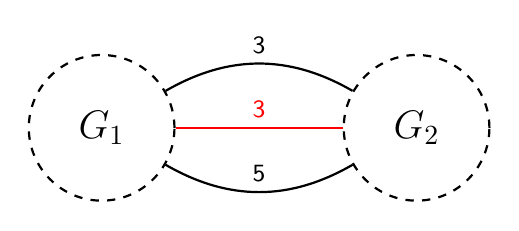
\begin{tikzpicture}[auto,node distance=3cm, every loop/.style={},thick,main node/.style={circle,draw,font=\sffamily\Large}]
                \node[main node, dashed] at (-2, 0) (g1) {\parbox{1.5cm}{\centering $G_1$}};

                \node[main node, dashed] at (2, 0) (g2) {\parbox{1.5cm}{\centering $G_2$}};

                \path[every node/.style={font=\sffamily\small}]
					(g1) edge[red] node [above] {3} (g2)
					(g1) edge[bend left] node [above] {3} (g2)
					(g1) edge[bend right] node [above] {5} (g2)
                    ;
            \end{tikzpicture}
            \caption{Árvore geradora mínima $T$ representada em vermelho no grafo $G'$ condensado}
            \label{mst}
        \end{figure}

		\begin{figure}[H]
			\centering
			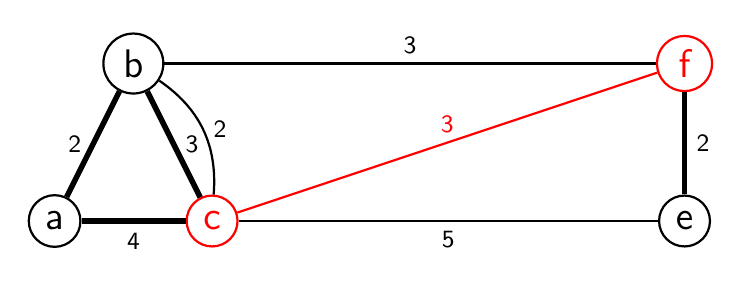
\begin{tikzpicture}[auto,node distance=3cm, every loop/.style={},thick,main node/.style={circle,draw,font=\sffamily\Large}]
				\node[main node] at (-5, -1) (a) {a};
				\node[main node] at (-4, 1) (b) {b};
				\node[main node, red] at (-3, -1) (c) {c};
				\node[main node] at (3, -1) (e) {e};
				\node[main node, red] at (3, 1) (f) {f};

				\path[every node/.style={font=\sffamily\small}]
					(a) edge[line width=2] node [left] {2} (b)
					(b) edge[line width=2] node [right] {3} (c)
					(b) edge[bend left] node [right] {2} (c)
					(a) edge[line width=2] node [below] {4} (c)
					(b) edge node [above] {3} (f)
					(c) edge node [below] {5} (e)
					(e) edge[line width=2] node [right] {2} (f)
					(c) edge[red] node [above] {3} (f)
					;
			\end{tikzpicture}
			\caption{Representação de $T$ em $G'$}
			\label{mst-2}
		\end{figure}

        \item[\textbf{Passo 2.}]
            Encontrar um emparelhamento perfeito $M$ de custo mínimo entre os vértices de grau ímpar do grafo induzido por $R \cup T$.

            No exemplo, os únicos vértices de grau ímpar em $R \cup T$ são os vértices $c$ e $e$.

        \begin{figure}[H]
            \centering
            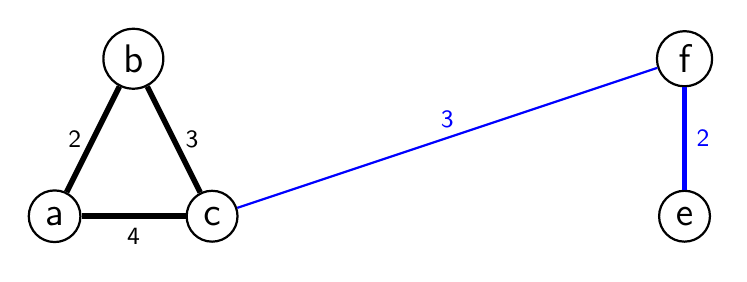
\begin{tikzpicture}[auto,node distance=3cm, every loop/.style={},thick,main node/.style={circle,draw,font=\sffamily\Large}]
                \node[main node] at (-5, -1) (a) {a};
                \node[main node] at (-4, 1) (b) {b};
                \node[main node] at (-3, -1) (c) {c};
                \node[main node] at (3, -1) (e) {e};
                \node[main node] at (3, 1) (f) {f};

                \path[every node/.style={font=\sffamily\small}]
                    (a) edge[line width=2] node [left] {2} (b)
                    (b) edge[line width=2] node [right] {3} (c)
                    (a) edge[line width=2] node [below] {4} (c)
                    (e) edge[blue, line width=2] node [right] {2} (f)
                    (c) edge[blue] node [above] {3} (f)
                    ;
            \end{tikzpicture}
            \caption{Grafo induzido por $R \cup T$ evidenciando o emparelhamento dos vértices $c$ e $e$ de custo mínimo}
            \label{mst-3}
        \end{figure}


        \item[\textbf{Passo 3.}]
            Encontrar um circuito euleriano no grafo induzido por $R \cup T \cup M$. 
            A partir de tal circuito é possível derivar-se um circuito de mesmo custo no grafo $G$ original que resolve o PCR.

        \begin{figure}[H]
            \centering
            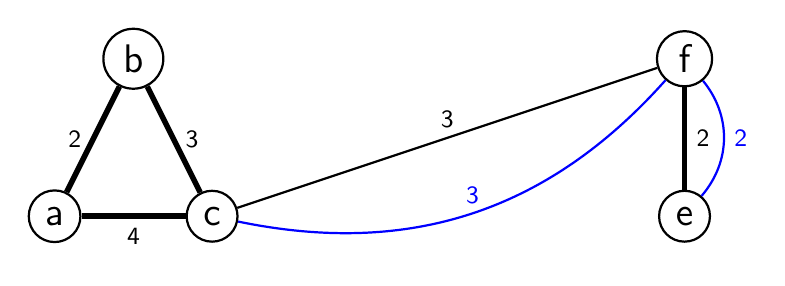
\begin{tikzpicture}[auto,node distance=3cm, every loop/.style={},thick,main node/.style={circle,draw,font=\sffamily\Large}]
                \node[main node] at (-5, -1) (a) {a};
                \node[main node] at (-4, 1) (b) {b};
                \node[main node] at (-3, -1) (c) {c};
                \node[main node] at (3, -1) (e) {e};
                \node[main node] at (3, 1) (f) {f};

                \path[every node/.style={font=\sffamily\small}]
                    (a) edge[line width=2] node [left] {2} (b)
                    (b) edge[line width=2] node [right] {3} (c)
                    (a) edge[line width=2] node [below] {4} (c)
                    (e) edge[line width=2] node [right] {2} (f)
                    (e) edge[blue, bend right=40] node [right] {2} (f)
                    (c) edge[] node [above] {3} (f)
                    (c) edge[blue, bend right] node [above] {3} (f)
                    ;
            \end{tikzpicture}
            \caption{Grafo induzido por $R \cup T \cup M$}
            \label{grafo-rtm}
        \end{figure}

        \begin{figure}[H]
            \centering
            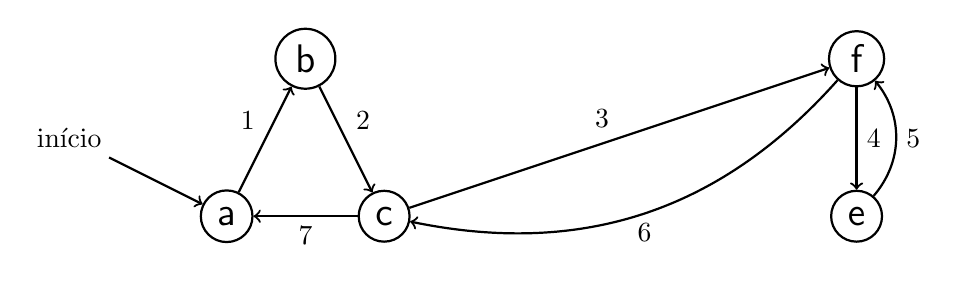
\begin{tikzpicture}[auto,node distance=3cm, every loop/.style={},thick,main node/.style={circle,draw,font=\sffamily\Large}]
                \node[main node] at (-5, -1) (a) {a};
                \node[main node] at (-4, 1) (b) {b};
                \node[main node] at (-3, -1) (c) {c};
                \node[main node] at (3, -1) (e) {e};
                \node[main node] at (3, 1) (f) {f};
                \node at(-7, 0) (st) {início};
                \path[->] (st) edge[] node {} (a);
                \path[->] (a) edge node {1} (b);
                \path[->] (b) edge node {2} (c);
                \path[->] (c) edge node {3} (f);
                \path[->] (f) edge node {4} (e);
                \path[->] (e) edge[bend right=40] node [right] {5} (f);
                \path[->] (f) edge[bend left] node[below] {6} (c);
                \path[->] (c) edge node {7} (a);

            \end{tikzpicture}
            \caption{Circuito euleriano em $R\cup T \cup M$}
            \label{circuito-euleriano}
        \end{figure}

        Segue agora o caminho que resolve o PCR no grafo original baseado no circuito euleriano da figura \ref{circuito-euleriano}:

        \begin{figure}[H]
            \centering
            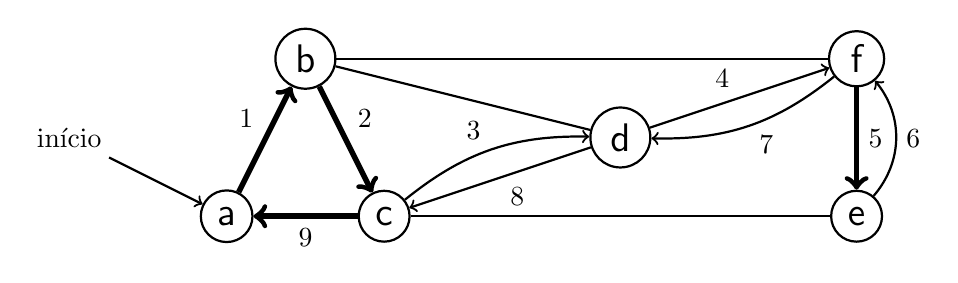
\begin{tikzpicture}[auto,node distance=3cm, every loop/.style={},thick,main node/.style={circle,draw,font=\sffamily\Large}]
                \node[main node] at (-5, -1) (a) {a};
                \node[main node] at (-4, 1) (b) {b};
                \node[main node] at (-3, -1) (c) {c};
                \node[main node] at (0, 0) (d) {d};
                \node[main node] at (3, -1) (e) {e};
                \node[main node] at (3, 1) (f) {f};
                \node at(-7, 0) (st) {início};
                \path[->] (st) edge[] node {} (a);
                \path[->] (a) edge[line width=2] node {1} (b);
                \path[->] (b) edge[line width=2] node {2} (c);
                \path[->] (c) edge[bend left=20] node {3} (d);
                \path[->] (d) edge node {4} (f);
                \path[->] (f) edge[line width=2] node {5} (e);
                \path[->] (e) edge[bend right=40] node [right] {6} (f);
                \path[->] (f) edge[bend left=20] node {7} (d);
                \path[->] (d) edge[] node {8} (c);
                \path[->] (c) edge[line width=2] node {9} (a);

                \path[every node/.style={font=\sffamily\small}]
                    (b) edge node [above] {} (d)
                    (b) edge node [above] {} (f)
                    (c) edge node [below] {} (e)
                    ;
            \end{tikzpicture}
            \caption{Solução do PCR encontrada pela heurística de Christofides}
            \label{sol-pcr}
        \end{figure}


        \end{enumerate}

        \subsubsection{PCR em grafos direcionados}

        Para tratar sobre a versão direcionada do PCR, tomaremos $G = (V, A)$ como o digrafo original e um conjunto $R \subseteq A$ de arcos que devem ser percorridos no circuito que resolve o PCR para $G$.

        Assim como no PCR para grafos não direcionados, a solução deste caso se baseia em estender o digrafo $G$ em um digrafo euleriano, cujo circuito euleriano representa uma solução para o PCR do digrafo original $G$.

        Será apresentada agora uma heurística que resolve esse problema, proposta por Christofides \cite{christofides-86}, muito semelhente à heurística apresentada para o caso de grafos não direcionados.

        \textbf{Heurística da arborescência geradora mínima}

        Para guiar a explicação da heurística toma-se, como exemplo, o digrafo $G$, a seguir:
   

        \begin{figure}[H]
            \centering
            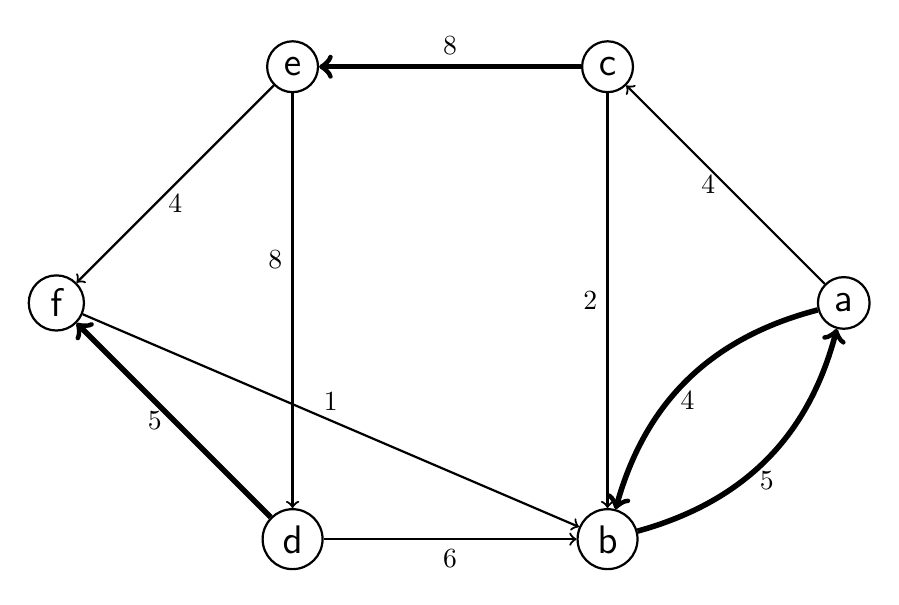
\begin{tikzpicture}[node distance=3cm, every loop/.style={},thick,main node/.style={circle,draw,font=\sffamily\Large}]

                \node[main node] at (-5, 0) (f) {f};
                \node[main node] at (-2, 3) (e) {e};
                \node[main node] at (2, 3) (c) {c};
                \node[main node] at (5, 0) (a) {a};
                \node[main node] at (-2, -3) (d) {d};
                \node[main node] at (2, -3) (b) {b};

                \path[->] (a) edge[line width=2, bend right, below] node {4} (b);
                \path[->] (a) edge[left] node {4} (c);
                \path[->] (b) edge[line width=2, below, bend right] node {5} (a);
                \path[->] (c) edge[line width=2, above] node {8} (e);
                \path[->] (c) edge[above, left] node {2} (b);
                \path[->] (d) edge[below] node {6} (b);
                \path[->] (d) edge[line width=2, left] node {5} (f);
                \path[->] (e) edge[below] node {4} (f);
                \path[->] (e) edge[pos=0.4, left] node {8} (d);
                \path[->] (f) edge[above] node {1} (b);
            \end{tikzpicture}
            \caption{Digrafo $G$, o conjunto $R$ corresponde aos arcos em negrito}
            \label{pcr-digraph}
        \end{figure}

        A extensão de $G$ em um digrafo euleriano $G' = (V', A')$ se dá de modo similar àquela do caso com grafos não direcionados:

        O conjunto de vértices possui a mesma definição, $V' = \{u \in V : (u, v) \in R \text{ para algum } v \in V\}$. 

        Como no grafo da figura \ref{pcr-digraph} todos vértices possuem ao menos um arco pertencente a $R$, define-se $V' = V$.

        De modo semelhante, o conjunto de arcos $A'$ será inicialmente acrescido dos arcos $(v_i, v_j)$ para todo par $v_i, v_j \in V'$, de custo igual ao custo do menor caminho de $v_i$ a $v_j$.
        Posteriormente remove-se de $A'$ todo arco que pertence também a $A \setminus R$ e cujo custo $c_{uv}$ é igual a $c_{uw} + c_{wv}$ para algum vértice $w$, removem-se também os arcos paralelos de mesmo valor que pertencem a $A \setminus R$.

        Realizando tal extensão no exemplo sugerido, teremos o digrafo $G'$ representado na figura \ref{extensionG}.

        \begin{figure}[H]
            \centering
            \scalebox{.8}{
                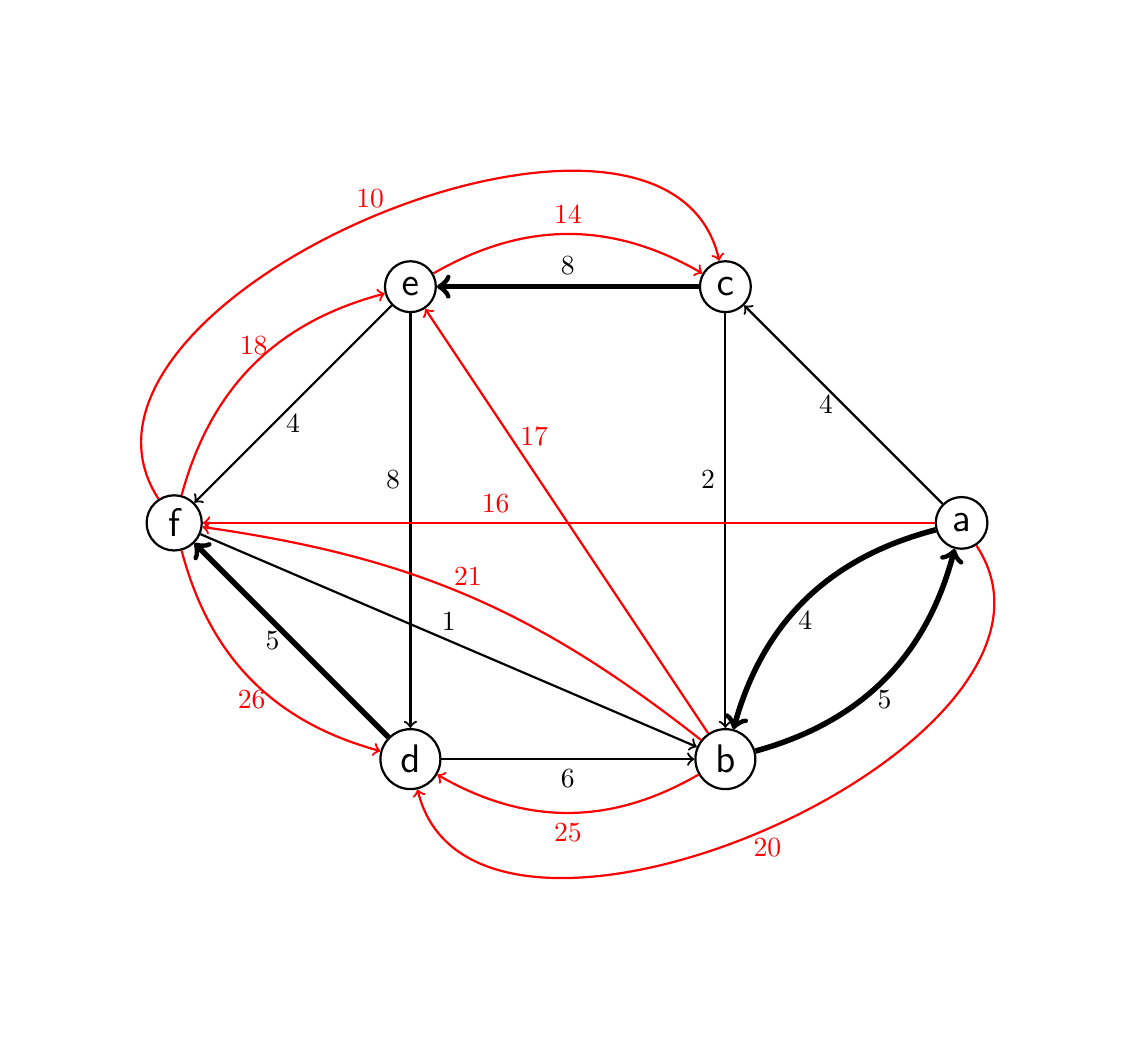
\begin{tikzpicture}[every loop/.style={},thick,main node/.style={circle,draw,font=\sffamily\Large}]

                    \node[main node] at (-5, 0) (f) {f};
                    \node[main node] at (-2, 3) (e) {e};
                    \node[main node] at (2, 3) (c) {c};
                    \node[main node] at (5, 0) (a) {a};
                    \node[main node] at (-2, -3) (d) {d};
                    \node[main node] at (2, -3) (b) {b};

                    \path[->] (a) edge[line width=2, bend right, below] node {4} (b);
                    \path[->] (a) edge[left] node {4} (c);
                    \path[->] (b) edge[line width=2, below, bend right] node {5} (a);
                    \path[->] (c) edge[line width=2, above] node {8} (e);
                    \path[->] (c) edge[above, left, pos=0.4] node {2} (b);
                    \path[->] (d) edge[below] node {6} (b);
                    \path[->] (d) edge[line width=2, left] node {5} (f);
                    \path[->] (e) edge[below] node {4} (f);
                    \path[->] (e) edge[pos=0.4, left] node {8} (d);
                    \path[->] (f) edge[above] node {1} (b);
                    \path[->] (a) edge[red, below, bend left=100] node {20} (d);
                    \path[->] (a) edge[red, above, pos=0.6] node {16} (f);
                    \path[->] (b) edge[bend left, red, below] node {25} (d);
                    \path[->] (b) edge[red, right, pos=0.7] node {17} (e);
                    \path[->] (b) edge[red, above, bend right=15] node {21} (f);
                    \path[->] (e) edge[red, bend left, above] node {14} (c);
                    \path[->] (f) edge[red, above, bend left=100] node {10} (c);
                    \path[->] (f) edge[red, below, bend right] node {26} (d);
                    \path[->] (f) edge[red, above, bend left] node {18} (e);
                \end{tikzpicture}
            }
            \caption{São vermelhas as arestas criadas na extensão $G'$}
            \label{extensionG}
        \end{figure}
		O grafo $G'$ será composto por $k$ conjuntos conexos $G_1, G_2, \dots, G_k$, induzidos por $R$. 
		Isto é, cada conjunto $G_i$ será composto apenas por arcos pertencentes a $R$ e será conexo, mas não necessariamente fortemente conexo.

        No exemplo apresentado, $G$ possui três componentes, $G_1$ composta pelos vértices $a, b$, $G_2$ composta por $c, e$ e $G_3$ composta por $d, f$.


	\begin{enumerate}
        \item[\textbf{Passo 1.}] 
			Encontrar uma arborescência geradora $T$ de custo mínimo que conecte os subgrafos $G_1, \dots, G_k$ e tem raiz em um vértice qualquer.

            Para encontrar tal arborescência, pode-se utilizar o algoritmo proposto independentemente pela dupla Yoeng-Jin Chu e Tseng-Hong Liu e por Edmonds\cite{edmonds-ssa}, sendo, portanto, chamado de algoritmo de Chu-Liu/Edmonds.

            Condensando o digrafo $G'$ em suas components $G_1, G_2, G_3$ temos o grafo representado na figura \ref{condensated-dig}.


            \begin{figure}[H]
                \centering
                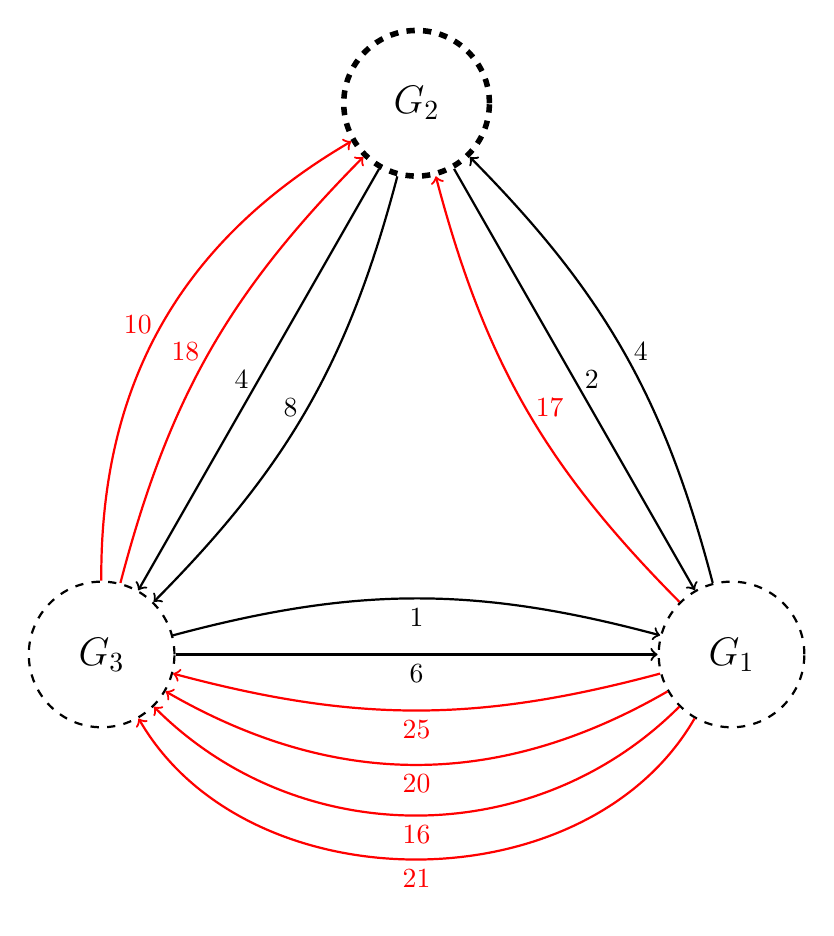
\begin{tikzpicture}[node distance=3cm, every loop/.style={},thick,main node/.style={circle,draw,font=\sffamily\Large}]

                    \node[main node, dashed] at (4, -4) (g1) {\parbox{1.5cm}{\centering $G_1$}};
                    \node[main node, dashed, line width=2] at (0, 3) (g2) {\parbox{1.5cm}{\centering $G_2$}};
                    \node[main node, dashed] at (-4, -4) (g3) {\parbox{1.5cm}{\centering $G_3$}};


                    \path[->] (g3) edge[below] node {6} (g1);
                    \path[->] (g3) edge[below, bend left=15] node {1} (g1);
                    \path[->] (g1) edge[below, bend left=15, red] node {25} (g3);
                    \path[->] (g1) edge[below, bend left, red] node {20} (g3);
                    \path[->] (g1) edge[below, bend left=45, red] node {16} (g3);
                    \path[->] (g1) edge[below, bend left=60, red] node {21} (g3);
                    \path[->] (g3) edge[left, bend left=15, red] node {18} (g2);
                    \path[->] (g3) edge[left, bend left, red] node {10} (g2);
                    \path[->] (g2) edge[left] node {4} (g3);
                    \path[->] (g2) edge[bend left=15, left] node {8} (g3);
                    \path[->] (g2) edge[right] node {2} (g1);
                    \path[->] (g1) edge[right, red, bend left=15] node {17} (g2);
                    \path[->] (g1) edge[right, bend right=15] node {4} (g2);

                \end{tikzpicture}
                \caption{Digrafo $G'$ condensado em suas componentes induzidas por $R$}
                \label{condensated-dig}
            \end{figure}

                O primeiro passo do algoritmo de Chu-Liu/Edmonds consiste em definir um vértice raiz $r$ para a arborescência.
                Como a heurística de Christofides não requer que um vértice específico seja tal raiz, podemos escolher o vértice condensado $G_1$ para cumprir tal função ($r = G_1$). 

                Definida a raiz $r$, deve-se retirar do digrafo analisado todos arcos que tem como destino $r$.
                Além disso, pode-se também substituir qualquer conjunto de arcos paralelos por um único arco com custo igual ao menor custo dos arcos paralelos removidos. 
                Pode-se visualizar o efeito de tais modificações em $G'$ na figura \ref{chu-liu}.

            \begin{figure}[H]
                \centering
                \scalebox{.7}{
                    \begin{tikzpicture}[node distance=3cm, every loop/.style={},thick,main node/.style={circle,draw,font=\sffamily\Large}]

                        \node[main node, dashed] at (4, -4) (g1) {\parbox{2cm}{\centering $r = G_1$}};
                        \node[main node, dashed, line width=2] at (0, 3) (g2) {\parbox{1.5cm}{\centering $G_2$}};
                        \node[main node, dashed] at (-4, -4) (g3) {\parbox{1.5cm}{\centering $G_3$}};


                        \path[->] (g1) edge[below, red] node {16} (g3);
                        \path[->] (g3) edge[left, bend left=10, red] node {10} (g2);
                        \path[->] (g2) edge[left, bend left=10] node {4} (g3);
                        \path[->] (g1) edge[right] node {4} (g2);

                    \end{tikzpicture}
                }
                \caption{Digrafo $G'$ após a remoção de arcos sugeridas pelo algoritmo de Chu-Liu/Edmonds}
                \label{chu-liu}
            \end{figure}

            Para todo vértice $v$ do grafo condensado diferente da raiz ($v \neq r$) encontra-se o arco de menor custo que chega em $v$.
            Define-se como $\pi(v)$ o vértice origem de tal arco.

            Se o conjunto de arcos $T = \{(\pi(v), v) | v \neq r\}$ não contém circuitos, então $T$ é uma arborescência de custo mínimo enraizada em $r$.
            Do contrário, realiza-se uma contração dos circuitos existentes em $T$, atualizam-se os custos dos arcos e repete-se recursivamente o mesmo procedimento de criação de $T$.

            No exemplo analisado, o conjunto $T$ consiste nos arcos de $G_1$ a $G_2$ e $G_2$ a $G_3$, ambos de custo 4.

            \begin{figure}[H]
                \centering
                \scalebox{.7}{
                    \begin{tikzpicture}[node distance=3cm, every loop/.style={},thick,main node/.style={circle,draw,font=\sffamily\Large}]

                        \node[main node, dashed] at (4, -4) (g1) {\parbox{2cm}{\centering $r = G_1$}};
                        \node[main node, dashed, line width=2] at (0, 3) (g2) {\parbox{1.5cm}{\centering $G_2$}};
                        \node[main node, dashed] at (-4, -4) (g3) {\parbox{1.5cm}{\centering $G_3$}};


                        \path[->] (g1) edge[below, red] node {16} (g3);
                        \path[->] (g3) edge[left, bend left=10, red] node {10} (g2);
                        \path[->] (g2) edge[blue, left, bend left=10] node {4} (g3);
                        \path[->] (g1) edge[blue, right] node {4} (g2);

                    \end{tikzpicture}
                }
            \caption{Em azul representa-se o conjunto de arcos $T$ definidos pelo algoritmo de Chu-Liu/Edmonds.}
            \label{chu-liu-p}
            \end{figure}


            Como $T$ não possui circuitos, não é necessário realizar uma nova iteração do algoritmo.
            $T$ é o conjunto de arcos que induz a arborescência de custo mínimo enraizada em $G_1$.

            Define-se como $R \cup T$ o digrafo induzido pelos arcos de $R$ e da arborescência $T$.


        \begin{figure}[H]
            \centering
            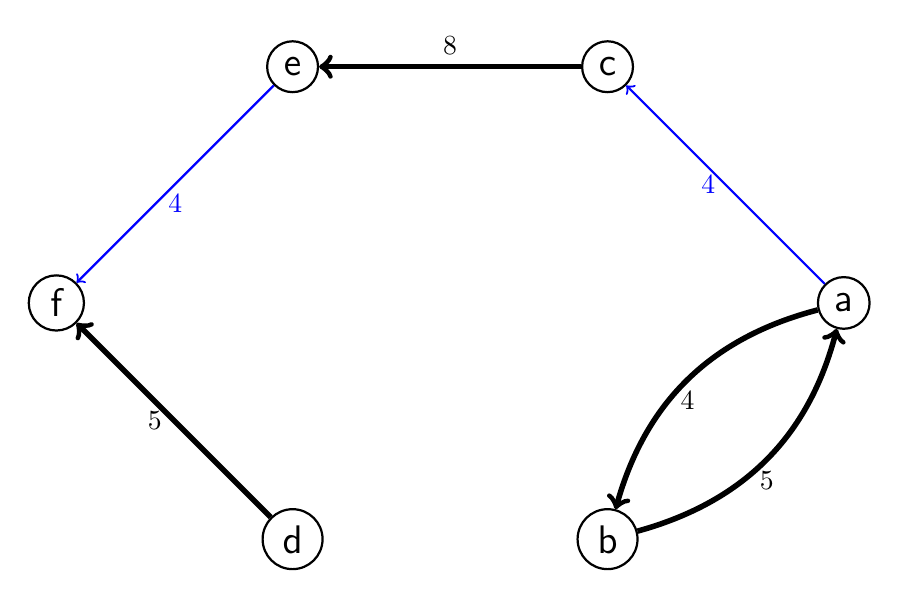
\begin{tikzpicture}[node distance=3cm, every loop/.style={},thick,main node/.style={circle,draw,font=\sffamily\Large}]

                \node[main node] at (-5, 0) (f) {f};
                \node[main node] at (-2, 3) (e) {e};
                \node[main node] at (2, 3) (c) {c};
                \node[main node] at (5, 0) (a) {a};
                \node[main node] at (-2, -3) (d) {d};
                \node[main node] at (2, -3) (b) {b};

                \path[->] (a) edge[line width=2, bend right, below] node {4} (b);
                \path[->] (a) edge[blue, left] node {4} (c);
                \path[->] (b) edge[line width=2, below, bend right] node {5} (a);
                \path[->] (c) edge[line width=2, above] node {8} (e);
                \path[->] (d) edge[line width=2, left] node {5} (f);
                \path[->] (e) edge[blue, below] node {4} (f);
            \end{tikzpicture}
            \caption{Digrafo $R\cup T$, os arcos de $T$ são representados em azul}
            \label{graphRUT}
        \end{figure}


        \item[\textbf{Passo 2.}]
            Encontrar um multiconjunto $M$ de menor custo composto por arcos de $A'$ que torna o digrafo induzido por $R \cup T$ euleriano, ou seja iguala os graus de entrada e saída de todos vértices.

			Pode-se determinar $M$ a partir da resolução de um problema de transporte: 
            O problema de transporte será definido tendo como base o grafo $G'$, porém as funções de oferta e demanda são definidas a partir dos graus dos vértices no grafo induzido por $R \cup T$.

            Um vértice $v \in V(G')$ cujo grau de entrada é maior que seu grau de saída (em relação ao subgrafo $R \cup T$) possuirá uma oferta igual ao valor absoluto da diferença de seus graus, do contrário, o valor absoluto da diferença representará a demanda do vértice $v$.

            No exemplo abordado, figura \ref{graphRUT}, o vértice $f$ possui uma oferta de valor $2$, os vértices $a$ e $d$ possuem uma demanda de valor $1$ e os vértices restantes já se encontram em igualdade de grau de entrada e saída.

			A resolução do problema de transporte modelado gera um conjunto de caminhos, representando a distribuição ótima da oferta. 
            O multiconjunto dos arcos pertencentes a união dos caminhos que solucionam o problema é o multiconjunto $M$ desejado.

            Sendo assim, como apenas uma origem existe no problema apresentado como exemplo, a solução do mesmo consiste na utilização dos caminhos de menor custo de $f$ a $a$ e de $f$ a $d$. 

        \begin{figure}[H]
            \centering
            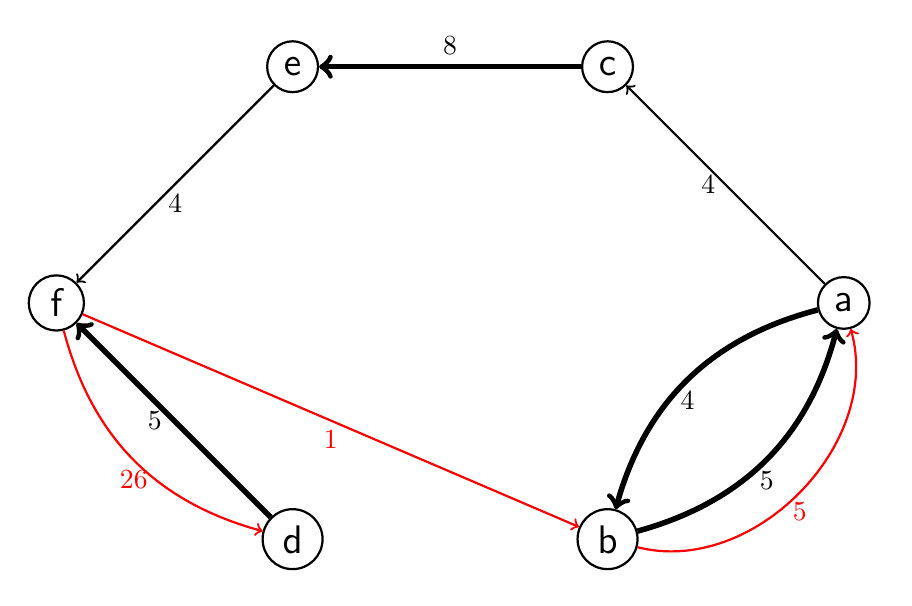
\begin{tikzpicture}[node distance=3cm, every loop/.style={},thick,main node/.style={circle,draw,font=\sffamily\Large}]

                \node[main node] at (-5, 0) (f) {f};
                \node[main node] at (-2, 3) (e) {e};
                \node[main node] at (2, 3) (c) {c};
                \node[main node] at (5, 0) (a) {a};
                \node[main node] at (-2, -3) (d) {d};
                \node[main node] at (2, -3) (b) {b};

                \path[->] (a) edge[line width=2, bend right, below] node {4} (b);
                \path[->] (a) edge[left] node {4} (c);
                \path[->] (b) edge[line width=2, below, bend right] node {5} (a);
                \path[->] (c) edge[line width=2, above] node {8} (e);
                \path[->] (d) edge[line width=2, left] node {5} (f);
                \path[->] (e) edge[below] node {4} (f);

                \path[->] (f) edge[red, below] node {1} (b);
                \path[->] (b) edge[red, below, bend right=60] node {5} (a);
                \path[->] (f) edge[red, bend right, below] node {26} (d);
            \end{tikzpicture}
            \caption{Digrafo euleriano $R\cup T \cup M$ com arcos de $M$ representados em vermelho.}
            \label{graphRUTUM}
        \end{figure}

        Na figura \ref{graphRUTUM} pode-se visualizar o digrafo induzido pelos arcos $R\cup T \cup M$. 
        Note que o arco de $b$ a $a$ de custo 5 é representado duas vezes, isso pois ele pertence tanto a $R$ quanto a $M$.

        \item[\textbf{Passo 3.}]
			O digrafo induzido pelo multiconjunto de arcos $R \cup T \cup M$ é, pela definição de $M$, euleriano. 
			
			Portanto, pode-se derivar um circuito euleriano de tal grafo. Por sua vez, a partir deste circuito, é possível derivar uma solução do PCR para o grafo original $G$.

            Um possível circuito euleriano para o exemplo apresentado é representado na figura \ref{circ-eulerianoRUTUM} a seguir.


        \begin{figure}[H]
            \centering
            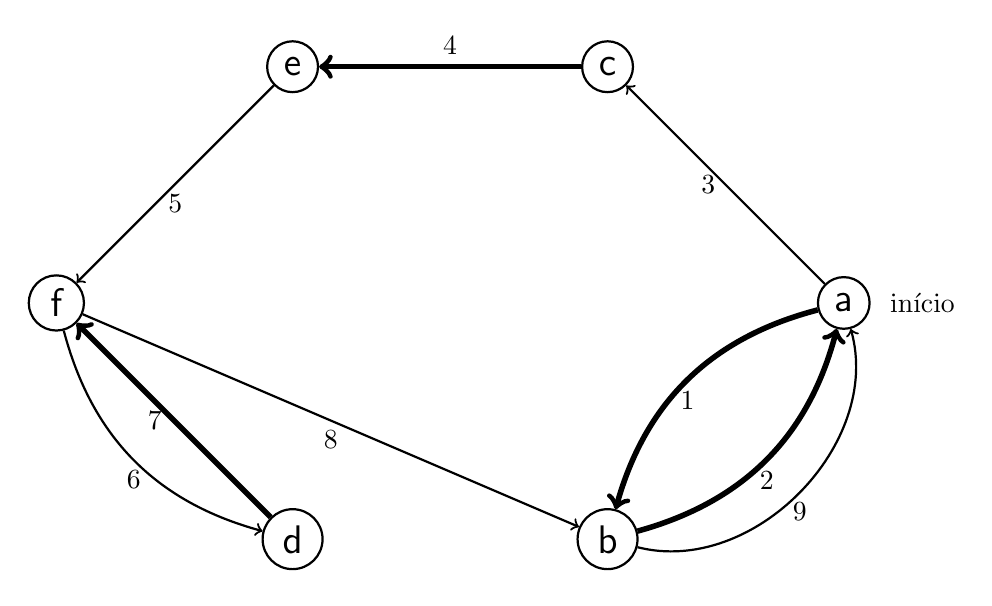
\begin{tikzpicture}[node distance=3cm, every loop/.style={},thick,main node/.style={circle,draw,font=\sffamily\Large}]

                \node[main node] at (-5, 0) (f) {f};
                \node[main node] at (-2, 3) (e) {e};
                \node[main node] at (2, 3) (c) {c};
                \node[main node] at (5, 0) (a) {a};
                \node at (6, 0) (ini) {início};
                \node[main node] at (-2, -3) (d) {d};
                \node[main node] at (2, -3) (b) {b};

                \path[->] (a) edge[line width=2, bend right, below] node {1} (b);
                \path[->] (b) edge[line width=2, below, bend right] node {2} (a);
                \path[->] (a) edge[left] node {3} (c);
                \path[->] (c) edge[line width=2, above] node {4} (e);
                \path[->] (e) edge[below] node {5} (f);
                \path[->] (f) edge[bend right, below] node {6} (d);
                \path[->] (d) edge[line width=2, left] node {7} (f);
                \path[->] (f) edge[below] node {8} (b);
                \path[->] (b) edge[below, bend right=60] node {9} (a);
            \end{tikzpicture}
            \caption{Circuito euleriano de $R\cup T \cup M$.}
            \label{circ-eulerianoRUTUM}
        \end{figure}

        A partir de tal circuito pode-se encontrar uma solução para o PCR do digrafo original $G$ expandindo os arcos contraídos na construção de $G'$ e removendo as duplicatas de arcos criados no procedimento da heurística.
        Por exemplo, o arco do nó $f$ ao $d$ de custo $26$ pertencente a $M$ consiste na condensação do caminho mínimo de $f$ a $d$: $\{f, b, a, c, e, d\}$.

        Realizando a remoção dos arcos artificiais adicionados a $G$ chegamos no seguinte circuito, baseado no circuito euleriano mostrado na figura \ref{circ-eulerianoRUTUM}:

        \begin{figure}[H]
            \centering
            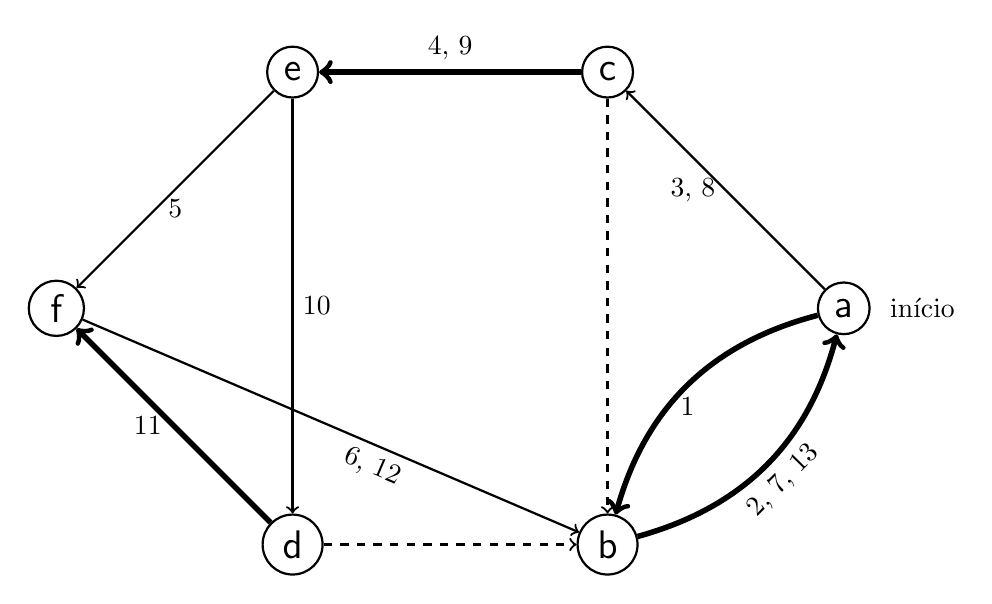
\begin{tikzpicture}[node distance=3cm, every loop/.style={},thick,main node/.style={circle,draw,font=\sffamily\Large}]

                \node[main node] at (-5, 0) (f) {f};
                \node[main node] at (-2, 3) (e) {e};
                \node[main node] at (2, 3) (c) {c};
                \node[main node] at (5, 0) (a) {a};
                \node at (6, 0) (ini) {início};
                \node[main node] at (-2, -3) (d) {d};
                \node[main node] at (2, -3) (b) {b};

                \path[->] (a) edge[line width=2, bend right, below] node {1} (b);
                \path[->] (b) edge[line width=2, below, bend right, sloped] node {2, 7, 13} (a);
                \path[->] (a) edge[left] node {3, 8} (c);
                \path[->] (c) edge[line width=2, above] node {4, 9} (e);
                \path[->] (e) edge[below] node {5} (f);

                \path[->] (e) edge[right] node {10} (d);

                \path[->] (d) edge[line width=2, left] node {11} (f);
                \path[->] (f) edge[pos=0.6, below, sloped] node {6, 12} (b);
                \path[->] (c) edge[dashed, above, left] node {} (b);
                \path[->] (d) edge[dashed, below] node {} (b);

            \end{tikzpicture}
            \caption{Construção de um circuito que resolve o PCR do grafo $G$. Representam-se em pontilhado os arcos de $G$ não percorridos na solução desenvolvida.}
            \label{solucaoPCR}
        \end{figure}
	\end{enumerate}

    Finaliza-se assim a execução da heurística da arborescência geradora mínima, que gera uma solução para o PCR de $G$ com custo 62.

    %TODO: Adicionar valor da solucao otima
    \subsection{Problema do carteiro chinês com vento}

        Considere o problema em que cada aresta tem um custo diferente dependendo do sentido em que é percorrida. Este problema é conhecido como o Problema do Carteiro Chinês com Vento (PCCV).

        Este problema possui várias aplicações. 
        Por exemplo, podem existir estradas com uma corrente de vento que o carteiro deve percorrer. 
        A corrente de vento tanto pode ajudar o carteiro se ele anda no mesmo sentido que a corrente, quanto pode atrapalhar o carteiro se ele anda no sentido contrário do vento.

        Outra ilustração possível para esta variação é imaginar que uma estrada pode ser inclinada, sendo assim mais difícil subir tal estrada do que descê-la.

        Esta variação do problema do carteiro chinês também é NP-difícil.

        Porém, como provado por Meigu Guan \cite{guan-windy}, se todo circuito de um grafo $G$ possui o mesmo custo independente do sentido em que é percorrido, então é possível encontrar uma solução para o PCCV usando um algoritmo polinomial, trataremos esse caso a seguir.

        Seja $c_{ij}$ o custo de se percorrer a aresta $ij$ de $i$ a $j$ e $c_{ji}$ o custo de percorrer a mesma aresta no sentido contrário.

        O algoritmo sugerido por Guan se baseia em criar uma nova função de custo $c'$ para o problema, tal que $c'_{ij} = c'_{ji} = \frac{c_{ij} + c_{ji}}{2}$ para toda aresta $ij$. 
        Essa transformação reduz o problema a um PCC não direcionado, que possui solução polinomial, como tratado na seção \ref{sec:pcc}.

        O teorema \ref{windy-theorem} enunciado a seguir, garante que uma resposta ótima do PCC no grafo $(G, c')$ equivale a uma resposta ótima, de mesmo custo, do PCCV no grafo original $(G, c)$.

        \begin{lemma}
            \label{lemma:pccv}
            Seja $G$ um grafo cujos circuitos possuem os mesmos custos independente do sentido em que são percorridos.
            Seja $C$ um circuito do grafo $G$, vale que:

            \[
                \sum_{ij \in C} c'_{ij} = \sum_{ij \in C} c'_{ji} =  \sum_{ij \in C} c_{ij} =  \sum_{ij \in C} c_{ji}
            \]
        \end{lemma}
        \begin{proof}
            Como $G$ respeita a propriedade que todo circuito possui custo igual, não importando a ordem em que o mesmo é percorrido, pode-se afirmar que:
            \[
                \sum_{ij \in C} c_{ij} =  \sum_{ij \in C} c_{ji}
            \]

            Além disso, por definição $c'_{ij} = c'_{ji}$, valendo assim que:
            \[
                \sum_{ij \in C} c'_{ij} = \sum_{ij \in C} c'_{ji} 
            \]

            Finalmente, pela definição de $c'$: 
            \begin{align*}
                \sum_{ij \in C} c'_{ij} &= \sum_{ij \in C} \frac{c_{ij} + c_{ji}}{2} \\
                \sum_{ij \in C} c'_{ij} &= \frac{1}{2} \left(\sum_{ij \in C}c_{ij} + \sum_{ij \in C}c_{ji} \right) \\
                \sum_{ij \in C} c'_{ij} &= \sum_{ij \in C} c_{ij}
            \end{align*}

        \end{proof}


        \begin{theorem}
            \label{windy-theorem}
            Seja $G$ um grafo conexo não direcionado cujos circuitos possuem o mesmo custo, independente do sentido que são percorridos. 

            Qualquer solução ótima para o PCC em $(G, c')$ também é uma solução ótima do PCCV em $(G, c)$.

        \end{theorem}

        Para exemplificar a prova deste teorema, usaremos o seguinte grafo $G$:
    
        \begin{figure}[H]
            \centering
            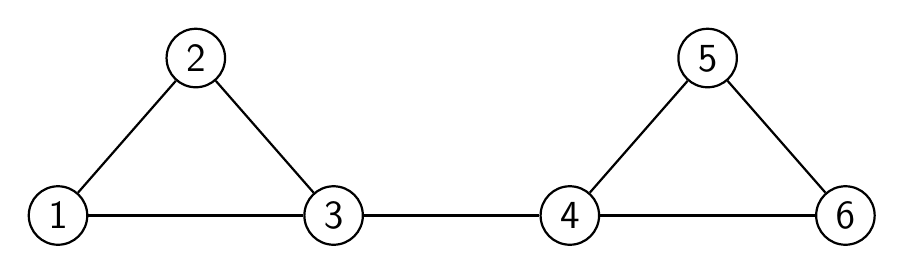
\begin{tikzpicture}[node distance=3cm, every loop/.style={},thick,main node/.style={circle,draw,font=\sffamily\Large}]
                \node[main node] at (-5, 0) (1) {1};
                \node[main node] at (-3.25, 2) (2) {2};
                \node[main node] at (-1.5, 0) (3) {3};
                \node[main node] at (1.5, 0) (4) {4};
                \node[main node] at (3.25, 2) (5) {5};
                \node[main node] at (5, 0) (6) {6};

            \path[-] (1) edge[] node {} (2);
            \path[-] (2) edge[] node {} (3);
            \path[-] (1) edge[] node {} (3);
            \path[-] (3) edge[] node {} (4);
            \path[-] (4) edge[] node {} (6);
            \path[-] (4) edge[] node {} (5);
            \path[-] (5) edge[] node {} (6);

            \end{tikzpicture}
            \caption{Grafo $G$}
            \label{goriginal}
        \end{figure}

        O custo de cada aresta será dado pela tabela \ref{tabela:exemplopccv}.

        \begin{table}[h!]
            \centering
            \begin{tabular}{|p{1.5cm}||p{1cm}|p{1cm}|p{1cm}|p{1cm}|p{1cm}|p{1cm}|}
                \hline
                    & \multicolumn{6}{|c|}{Destino} \\
                \hline
                   Origem & 1 & 2 & 3 & 4 & 5 & 6\\
                \hline
                \hline
                1 &  & 2 & 3 &  & & \\
                \hline
                2 & 5 &  & 3 & & & \\
                \hline
                3 & 4 & 1 & & 7 & & \\
                \hline
                4 &  & & 1 & & 1 & 1\\
                \hline
                5 &  & & & 3 & & 4\\
                \hline
                6 &  &  & & 2 & 3 &\\
                \hline
            \end{tabular}
            \caption{O custo de se percorrer a aresta de $i$ a $j$ é o valor da linha $i$ e coluna $j$}
            \label{tabela:exemplopccv}
    \end{table}
        
        Para melhor visualização destes custos, podemos representar o grafo original usando pares de arcos para cada aresta existente:

        \begin{figure}[H]
            \centering
            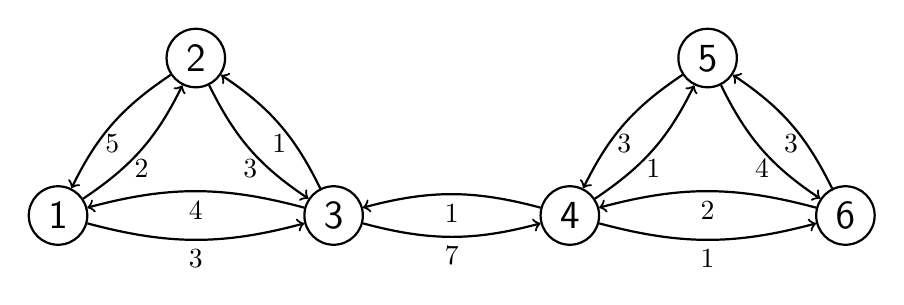
\begin{tikzpicture}[node distance=3cm, every loop/.style={},thick,main node/.style={circle,draw,font=\sffamily\Large}]
                \node[main node] at (-5, 0) (1) {1};
                \node[main node] at (-3.25, 2) (2) {2};
                \node[main node] at (-1.5, 0) (3) {3};
                \node[main node] at (1.5, 0) (4) {4};
                \node[main node] at (3.25, 2) (5) {5};
                \node[main node] at (5, 0) (6) {6};

            \path[->] (1) edge[bend right=15, below] node {2} (2);
            \path[->] (2) edge[bend right=15, below] node {5} (1);
            \path[->] (2) edge[bend right=15, below] node {3} (3);
            \path[->] (3) edge[bend right=15, below] node {1} (2);
            \path[->] (1) edge[bend right=15, below] node {3} (3);
            \path[->] (3) edge[bend right=15, below] node {4} (1);

            \path[->] (3) edge[bend right=15, below] node {7} (4);
            \path[->] (4) edge[bend right=15, below] node {1} (3);

            \path[->] (4) edge[bend right=15, below] node {1} (6);
            \path[->] (6) edge[bend right=15, below] node {2} (4);
            \path[->] (4) edge[bend right=15, below] node {1} (5);
            \path[->] (5) edge[bend right=15, below] node {3} (4);
            \path[->] (5) edge[bend right=15, below] node {4} (6);
            \path[->] (6) edge[bend right=15, below] node {3} (5);

            \end{tikzpicture}
            \caption{Representação direcionada do grafo $G$}
            \label{exGdir}
        \end{figure}

        Note que os dois circuitos dessa imagem possuem o mesmo custo independente do sentido em que são percorridos:

        \begin{figure}[H]
            \centering
            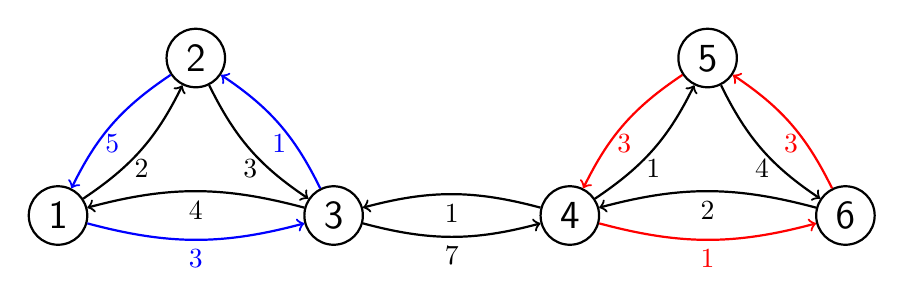
\begin{tikzpicture}[node distance=3cm, every loop/.style={},thick,main node/.style={circle,draw,font=\sffamily\Large}]
                \node[main node] at (-5, 0) (1) {1};
                \node[main node] at (-3.25, 2) (2) {2};
                \node[main node] at (-1.5, 0) (3) {3};
                \node[main node] at (1.5, 0) (4) {4};
                \node[main node] at (3.25, 2) (5) {5};
                \node[main node] at (5, 0) (6) {6};

            \path[->] (1) edge[bend right=15, below] node {2} (2);
            \path[->] (2) edge[blue, bend right=15, below] node {5} (1);
            \path[->] (2) edge[bend right=15, below] node {3} (3);
            \path[->] (3) edge[blue, bend right=15, below] node {1} (2);
            \path[->] (1) edge[blue, bend right=15, below] node {3} (3);
            \path[->] (3) edge[bend right=15, below] node {4} (1);

            \path[->] (3) edge[bend right=15, below] node {7} (4);
            \path[->] (4) edge[bend right=15, below] node {1} (3);

            \path[->] (4) edge[red, bend right=15, below] node {1} (6);
            \path[->] (6) edge[bend right=15, below] node {2} (4);
            \path[->] (4) edge[bend right=15, below] node {1} (5);
            \path[->] (5) edge[red, bend right=15, below] node {3} (4);
            \path[->] (5) edge[bend right=15, below] node {4} (6);
            \path[->] (6) edge[red, bend right=15, below] node {3} (5);

            \end{tikzpicture}
            \caption{Circuitos com custo $9$ e $7$ respectivamente}
        \end{figure}


        \begin{figure}[H]
            \centering
            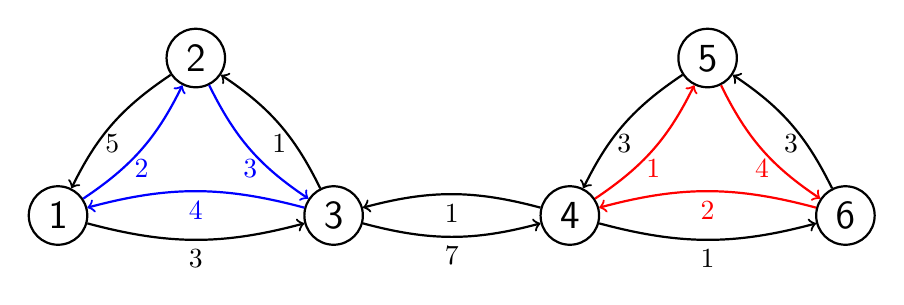
\begin{tikzpicture}[node distance=3cm, every loop/.style={},thick,main node/.style={circle,draw,font=\sffamily\Large}]
                \node[main node] at (-5, 0) (1) {1};
                \node[main node] at (-3.25, 2) (2) {2};
                \node[main node] at (-1.5, 0) (3) {3};
                \node[main node] at (1.5, 0) (4) {4};
                \node[main node] at (3.25, 2) (5) {5};
                \node[main node] at (5, 0) (6) {6};

            \path[->] (1) edge[blue, bend right=15, below] node {2} (2);
            \path[->] (2) edge[bend right=15, below] node {5} (1);
            \path[->] (2) edge[blue, bend right=15, below] node {3} (3);
            \path[->] (3) edge[bend right=15, below] node {1} (2);
            \path[->] (1) edge[bend right=15, below] node {3} (3);
            \path[->] (3) edge[blue, bend right=15, below] node {4} (1);

            \path[->] (3) edge[bend right=15, below] node {7} (4);
            \path[->] (4) edge[bend right=15, below] node {1} (3);

            \path[->] (4) edge[bend right=15, below] node {1} (6);
            \path[->] (6) edge[red,bend right=15, below] node {2} (4);
            \path[->] (4) edge[red,bend right=15, below] node {1} (5);
            \path[->] (5) edge[bend right=15, below] node {3} (4);
            \path[->] (5) edge[red, bend right=15, below] node {4} (6);
            \path[->] (6) edge[bend right=15, below] node {3} (5);

            \end{tikzpicture}
            \caption{Circuitos no sentido contrário com mesmo custo, $9$ e $7$}
        \end{figure}

        Realizando a transformação da função do custo de toda aresta $ij$ de $c_{ij}$ para $c'_{ij} = \frac{c_{ij} + c_{ji}}{2}$ temos a seguinte representação de $(G, c')$:


        \begin{figure}[H]
            \centering
            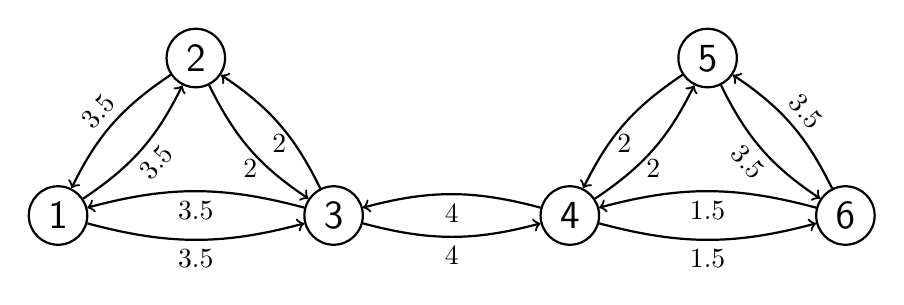
\begin{tikzpicture}[node distance=3cm, every loop/.style={},thick,main node/.style={circle,draw,font=\sffamily\Large}]
                \node[main node] at (-5, 0) (1) {1};
                \node[main node] at (-3.25, 2) (2) {2};
                \node[main node] at (-1.5, 0) (3) {3};
                \node[main node] at (1.5, 0) (4) {4};
                \node[main node] at (3.25, 2) (5) {5};
                \node[main node] at (5, 0) (6) {6};

            \path[->] (1) edge[bend right=15, below, sloped] node {3.5} (2);
            \path[->] (2) edge[bend right=15, sloped, above] node {3.5} (1);
            \path[->] (2) edge[bend right=15, below] node {2} (3);
            \path[->] (3) edge[bend right=15, below] node {2} (2);
            \path[->] (1) edge[bend right=15, below] node {3.5} (3);
            \path[->] (3) edge[bend right=15, below] node {3.5} (1);

            \path[->] (3) edge[bend right=15, below] node {4} (4);
            \path[->] (4) edge[bend right=15, below] node {4} (3);

            \path[->] (4) edge[bend right=15, below] node {1.5} (6);
            \path[->] (6) edge[bend right=15, below] node {1.5} (4);
            \path[->] (4) edge[bend right=15, below] node {2} (5);
            \path[->] (5) edge[bend right=15, below] node {2} (4);
            \path[->] (5) edge[bend right=15, sloped, below] node {3.5} (6);
            \path[->] (6) edge[bend right=15, sloped, above] node {3.5} (5);

            \end{tikzpicture}
            \caption{Representação direcionada do grafo $G$ com custos $c'$}
            \label{gclinha}
        \end{figure}

        Definido o exemplo que seguiremos, podemos seguir com a prova do teorema \ref{windy-theorem}

        \begin{proof} 
            Seja $T$ uma solução para o PCC em $(G, c')$. 
            $T$ será um passeio fechado composto por arestas orientadas de $G$.

            Pode-se dividir $T$ em circuitos de arcos $C_1, C_2, \dots, C_k$, com $k \in \mathbb{N}$ . % TODO: provar que pode dividir T em circuitos
            Podemos expressar o custo da solução $T$ como a soma dos custos de cada arco dos circuitos $C_1, C_2, \dots, C_k$. 

            Provaremos por indução, que para um circuito qualquer $C_i$ vale que:
            \[
                \sum_{ij \in C_i} c_{ij} = \sum_{ij \in C_i} c'_{ij}
            \]

            Seja $T = \{1, 2, 3, 4, 5, 6, 4, 3, 1\}$ uma solução ótima do PCCV do exemplo da figura \ref{gclinha}.
            Por si só, $T$ é um circuito de arcos, já que não percorre um mesmo arco duas vezes, mas para exemplificar melhor os casos a seguir decompomos $T$ em dois circuitos: $C_1 = \{1, 2, 3, 4, 3, 1\}, C_2 = \{4, 5, 6, 4\}$.

            A indução é realizada com base no tamanho do circuito $C_i$ analisado.

            Há dois casos base desta indução:

            \begin{itemize}
                \item Quando o circuito analisado $C_i$ é vazio.
                \item Quando $C_i$ é um circuito presente no grafo original $G$. 
                    Isto é, $C_i$ não percorre uma mesma aresta de $G$ mais que uma vez.
                    O lema \ref{lemma:pccv} garante a hipótese de igualdade neste caso.
            \end{itemize}

            No exemplo que estamos tratando, o circuito $C_2$ se enquadra no segundo tipo de caso base, já que $C_2 = \{4, 5, 6, 4\}$ está no grafo original \ref{goriginal}

            Assume-se que a hipótese de indução vale para circuitos com até $k$ arcos.

            Seja $C_i$ um circuito que não faz parte do caso base e que possui $k+1$ arcos.

            Pela definição de circuitos, $C_i$ não pode possuir arcos duplicados.  
            Sendo assim, para $C_i$ não estar presente em $G$, deverá existir uma aresta $uv$ de $G$ tal que $uv \in C_i$ e $vu \in C_i$, como representa-se a seguir:

            \[
                C_i = \{ w_1w_2, \dots, w_iu, uv, vw_{i+1}, \dots, w_jv,  vu, uw_{j+1}, \dots w_kw_1\}
            \]

            É possível, a partir de tal representação retirar de $C_i$ os arcos $uv$ e $vu$, separando-o em dois circuitos direcionados de tamanho menor:

            \[
                C'_i = \{w_1w_2, \dots w_iu, uw_{j+1}, \dots, w_kw_1\} 
            \]
            \[
                C''_i = \{vw_{i+1}, \dots, w_jv\}
            \]

            Como ambos novos circuitos tem tamanho menor que $|C_i| = k+1$, vale a hipótese para ambos:
            \begin{align}
                \sum_{ij \in C'_i} c_{ij} &= \sum_{ij \in C'_i} c'_{ij} \\
                \sum_{ij \in C''_i} c_{ij} &= \sum_{ij \in C''_i} c'_{ij}
            \end{align}
            
            Além disso, vale pela definição da função $c'$, que:
            
            \begin{align}
                c_{uv} + c_{vu}  &= c'_{uv} + c'_{vu} 
            \end{align}

            Somando as três igualdades apresentadas temos a representação do custo de $C_i$:

            \begin{align*}
                \sum_{ij \in C'_i} c_{ij} +  \sum_{ij \in C''_i} c_{ij} + c_{uv} + c_{vu}  &= \sum_{ij \in C'_i} c'_{ij} + \sum_{ij \in C''_i} + c'_{ij} c'_{uv} + c'_{vu}  \\
                \sum_{ij \in C_i} c_{ij} &= \sum_{ij \in C_i} c'_{ij} \\
            \end{align*}
             
            Provando assim que a hipótese de indução também vale para um circuito de tamanho $k+1$.

            Finalmente, temos que o custo da solução $T$ do PCCV de $(G, c)$ será igual ao custo da solução do PCC em $(G, c')$:

            \begin{align*}
                \sum_{ij \in T} c_{ij} &= \sum_{1 \leq u \leq k} \sum_{ij \in C_u} c_{ij} \\
                                       &= \sum_{1 \leq u \leq k} \sum_{ij \in C_u} c'_{ij} \\
                                       &= \sum_{ij \in T} c'_{ij} \\
            \end{align*}


            Voltando ao exemplo, temos agora que analisar o cirtcuito $C_1$.

            Apesar de $C_1$ ser um circuito válido na representação direcionada de $G$ (figura \ref{exGdir}), o mesmo não pode ser considerado um circuito do grafo não direcionado $G$ pois percorre a mesma aresta $(3 - 4)$ duas vezes, devemos portanto aplicar o passo da indução a $C_1$.
            
            Representando $C_1$ como um conjunto de arcos percorridos:

            \[
                C_1 = \{ 3\rightarrow 4, 4\rightarrow 5, 5\rightarrow 6, 6\rightarrow 4, 4\rightarrow 3 \}                
            \]

            Realizando a quebra de $C_1$ a partir dos arcos $3 \rightarrow 4$ e $4 \rightarrow 3$ temos:

            \[
                C'_1  = \{4 \rightarrow 5, 5\rightarrow 6, 6\rightarrow 4\}
            \]
            \[
                C''_1 = \{\}
            \] 

            Como $C'_1$ é um circuito presente no grafo original e $C''_1$ é um conjunto vazio, ambos são cobertos pelos casos base estabelecidos.

            Finalmente, pode-se comparar o custo da solução $T$ do PCCV de $G$ com as duas funções de custo definidas: $c$ e $c'$.

            \begin{align*}
                & T = \{ 1, 2, 3, 4, 5, 6, 4, 3, 1\} \\
                \sum_{ij \in T} c_{ij} &= c_{12} + c_{23} + c_{34} + c_{45} + c_{56} + c_{64} + c_{43} + c_{31} \\
                &= 2 + 3 + 7 + 1 + 4 + 2 + 1 + 4 \\
                &= 24 \\
                \sum_{ij \in T} c'_{ij} &= c'_{12} + c'_{23} + c'_{34} + c'_{45} + c'_{56} + c'_{64} + c'_{43} + c'_{31} \\
                &= 3.5 + 2 + 4 + 2 + 3.5 + 1.5 + 4 + 3.5 \\
                &= 24 \\
            \end{align*}

            Como provado, ambas funções de custo são equivalentes para o cálculo do custo da solução $T$.
        \end{proof}

%    \subsection{Problema do Carteiro Hierárquico}
%
%    Nesta variação são definidos $k$ subconjuntos de arestas $\{A_1, A_2, \dots, A_k\}$.
%    Como no problema do cartiro chinês original deve-se encontrar um passeio que passe por todas arestas de um grafo $G$, porém esse passeio só poderá percorrer uma aresta pertencente a um subconjunto $A_j$ se o mesmo já tiver percorrido todas arestas pertencentes aos conjuntos $A_i$ com $1 \leq i < j$.
%
%    Esta variação também é NP-difícil.
